\documentclass{article}

\usepackage{arxiv}

\usepackage[utf8]{inputenc} % allow utf-8 input
\usepackage[T1]{fontenc}    % use 8-bit T1 fonts
\usepackage{lmodern}        % https://github.com/rstudio/rticles/issues/343
\usepackage{hyperref}       % hyperlinks
\usepackage{url}            % simple URL typesetting
\usepackage{booktabs}       % professional-quality tables
\usepackage{amsfonts}       % blackboard math symbols
\usepackage{nicefrac}       % compact symbols for 1/2, etc.
\usepackage{microtype}      % microtypography
\usepackage{graphicx}

\title{Prevailing scenarios of functional change in Anthropocene bird
and mammal communities}

\author{
  }


% tightlist command for lists without linebreak
\providecommand{\tightlist}{%
  \setlength{\itemsep}{0pt}\setlength{\parskip}{0pt}}


% Pandoc citation processing
\newlength{\cslhangindent}
\setlength{\cslhangindent}{1.5em}
\newlength{\csllabelwidth}
\setlength{\csllabelwidth}{3em}
\newlength{\cslentryspacingunit} % times entry-spacing
\setlength{\cslentryspacingunit}{\parskip}
% for Pandoc 2.8 to 2.10.1
\newenvironment{cslreferences}%
  {}%
  {\par}
% For Pandoc 2.11+
\newenvironment{CSLReferences}[2] % #1 hanging-ident, #2 entry spacing
 {% don't indent paragraphs
  \setlength{\parindent}{0pt}
  % turn on hanging indent if param 1 is 1
  \ifodd #1
  \let\oldpar\par
  \def\par{\hangindent=\cslhangindent\oldpar}
  \fi
  % set entry spacing
  \setlength{\parskip}{#2\cslentryspacingunit}
 }%
 {}
\usepackage{calc}
\newcommand{\CSLBlock}[1]{#1\hfill\break}
\newcommand{\CSLLeftMargin}[1]{\parbox[t]{\csllabelwidth}{#1}}
\newcommand{\CSLRightInline}[1]{\parbox[t]{\linewidth - \csllabelwidth}{#1}\break}
\newcommand{\CSLIndent}[1]{\hspace{\cslhangindent}#1}

\usepackage{lineno}
\linenumbers
\usepackage{booktabs}
\usepackage{longtable}
\usepackage{array}
\usepackage{multirow}
\usepackage{wrapfig}
\usepackage{float}
\usepackage{colortbl}
\usepackage{pdflscape}
\usepackage{tabu}
\usepackage{threeparttable}
\usepackage{threeparttablex}
\usepackage[normalem]{ulem}
\usepackage{makecell}
\usepackage{xcolor}
\begin{document}
\maketitle


\begin{abstract}
Aim: Despite unprecedented environmental change due to anthropogenic
pressure, recent work has found increasing species turnover but no
overall trend in species diversity through time at the local scale.
Functional diversity provides a potentially powerful alternative
approach for understanding community composition by linking shifts in
species identity to mechanisms of ecosystem processes. Here we present
the first multi-taxa, multi-system analysis of functional change through
time.

Location: Global, with a North American focus

Time period: 1923-2014

Major taxa studied: Mammals, Birds

Methods: We paired thousands of bird and mammal assemblage time series
from the BioTIME database with existing trait data representative of a
species' functional role to reconstruct time series of functional
diversity metrics. Using generalized linear mixed models, we estimated
general trends in those metrics and trends for individual studies.

Results: We found no overall trend in any functional diversity metric,
despite data replicating species-based patterns of constant richness
with increasing turnover. The lack of trend held even after correcting
for changes in species richness. At the study-level, there were also a
substantial number of time series exhibiting no species or functional
change, however most studies showed a shift in a species or functional
metric.

Main Conclusions: General trends indicate that on the aggregate one type
of functional shift is not more prevalant than the other across many
taxa, biomes, and realms. At the study-level, we identified four
prevailing scenarios of species and functional change, which showed
links to the duration of the observation window. With no one prevailing
scenario of change, it will be critical to link change scenarios to
drivers of change, particularly to identify communities with capacity to
resist drivers from those not experiencing substantial pressure from a
driver.
\end{abstract}

\keywords{
    biodiversity change
   \and
    functional traits
   \and
    global change
   \and
    time series
  }

\hypertarget{introduction}{%
\section{Introduction}\label{introduction}}

Ecological communities are experiencing unprecedented change as a result
of anthropogenic pressures such as climate change, land use change, and
invasive species. Impacts of these pressures are well documented at a
global scale by an accelerating global extinction rate (1), and
fundamental changes in some of the most well-studied systems (e.g.~coral
bleaching, 2). At the local scale however, species diversity tells a
different story. Recent syntheses of local trends in biodiversity over
time have found no net change in local species diversity despite ongoing
turnover (3--6) and evidence of significant shifts in community
composition underlying consistent species richness (7--9). While
communities are clearly changing, our most common species-based
approaches do not fully capture the nature of that change.

The meaning of general trends derived from limited data, and their
relevance for conservation, is a topic of on going debate. Global
analyses have been heavily criticized for geographic biases, lack of
data in the most heavily impacted areas, and not considering the
ecological context of individual studies (10--12). Many of these
criticisms reflect limitations of ecological data on the whole, and
proponents argue we must make the best of the imperfect data available
(13). Still, there is general consensus on a few local-scale patterns
that seem to be characteristic of the anthropocene, including the
prevalence of species turnover across communities and patterns of both
richness increase and decrease in different taxa and biomes (14).
Understanding the implications of change in species assemblage for
ecosystem stability and function is a critical next step in moving
forward the biodiversity change conversation.

Functional diversity offers a potentially powerful alternative to
species-based approaches for detecting and describing community change
by providing a mechanistic link between species' response to
environmental change (\emph{response traits}) and the processes they
perform (\emph{effect traits}) (15--17). By describing the functional
trait space, functional diversity metrics capture the disproportionate
impact of losses or gains of functionally unique species. Functional
diversity metrics are therefore particularly well suited for assessing
community shifts underlying even constant species richness trends.

Beyond simply characterizing changes in community structure, trends in
functional composition also have important implications for ecosystem
stability, function, and resilience. There is increasing evidence
functional diversity is a better predictor of ecosystem function than
species-based metrics (18, 19), and that different facets of functional
diversity play essential roles in maintaining ecosystem stability (20,
21). Almost all hypothesized mechanisms underpinning the relationship
between species diversity and ecosystem function are trait-dependent
(22). Determining functional trends therefore gives a more direct
picture of potential trends in critical ecosystem processes.

It is critical to establish whether or not functional loss is prevalent
across communities. While functional loss is frequently cited as one of
the most pressing concerns of the anthropocene (23--25), local-scale
loss is not necessarily inevitable even in scenarios of species loss
(26, 27). Forecasts of functional loss range from negligible (28) to
dire (29, 30). And while some observed trends show significant
functional loss (31) others document no loss even in some of the most
heavily impacted communities (32--34). On paleoecological time scales
functional composition shows mixed responses to environmental change and
extinction events (35, 36), with significant impacts of species
extinctions on functional diversity in some taxa and not others (37).
For some time periods, functional structure appears to be maintained for
substantial portions of geological time (38). Still, some losses of
functional diversity are indisputable on both paleoecological and
contemporary timescales such as continued trophic downgrading due to
loss of large-bodied mammals, but implications of those losses for local
diversity patterns are less clear (39, 40) .

Assessments of broad-scale temporal change in functional diversity have
previously been limited by a lack of functional trait data. The majority
of work has therefore focused largely on system-specific studies with
traits collected \emph{in situ}. This has challenged our ability to
establish general rules for how functional composition may be changing
through time, particularly in response to global change drivers. Ongoing
efforts to assemble functional traits for a variety of taxa have made
synthesis of existing community assemblage data and functional traits
possible for the first time, providing initial insights into the ways
functional diversity changes on a broad scale for specific taxa
(e.g.~fish, 41, birds, 42, 43). However, to date there has been no
cross-taxa assessment of temporal functional change for a broad
geographic and taxonomic extent (44).

Here we perform the first multi-taxa, multi-realm assessment of
functional diversity change through time. We focus on mammal and bird
species as a significant subset of the world's biodiversity heavily
impacted by anthropogenic change. While examining trends in plants,
invertebrates, and other vertebrate species is of equal interest, trait
data for those taxa raise additional challenges such as limited and
biased species coverage (45), a lack of accepted species-level means,
and differences in the types of traits collected. To ensure
comparability across taxa in trait type and data quality we therefore
focus on mammals and birds. Traits were intentionally selected to be
representative of a species' Eltonian niche, thereby summarizing the
functional role they play in the community (46). An initial assessment
of amphibian trends is included in the supplement, but excluded from
general trend assessment here due to limited geographic coverage.

We assess thousands of mammal and bird functional diversity time series
to determine whether or not there is a general trend of functional
change, both in observed metrics and in metrics corrected for changes in
species richness. We further assess the prevailing modes of change
occurring at the study level to determine how functional change is
related to species patterns, and which kinds of species and functional
change are most common across communities. We expect to find significant
functional changes happening alongside and independent of species
richness changes as a result of ongoing anthropogenic impacts and global
change drivers.

\hypertarget{material-and-methods}{%
\section{Material and Methods}\label{material-and-methods}}

\hypertarget{data}{%
\subsection{Data}\label{data}}

We obtained mammal and bird time series from the BioTIME database, a
global repository of high-quality assemblage time series. All studies
included in the database follow consistent sampling protocols and
represent full assemblages rather than populations of single species
(36). All time series include abundance of observed species. Following
best practices for the database (47), studies with multiple sample
locations were split into individual time series following a
standardized spatial scale. Scale was set by a global grid with cell
size determined based on the sample extent of studies with only a single
location (see 36 for details on how sample extents were defined), with
the area of each cell set to one standard deviation away from the mean
of the single extent locations. All samples from a study within a single
cell were considered to be a single time series, and species abundances
were combined for all samples.

We used trait data from the Elton Trait Database, which consists of
species-level means for traits that represent species' multifaceted role
in the community (46). Traits include: body mass, diet, active diel
period, nocturnality, forest foraging strata, pelagic use. Multiple
traits (i.e.~diet, foraging strata, activity seasonality, active diel
period) were broken down into percentage or binary use for each level.

In order to ensure taxonomic consistency across datasets, BioTIME
species were paired with trait data based on their species identifier
from the Integrated Taxonomic Information System database (retrieved
09-15-2020 from the on-line database,
\url{https://doi.org/10.5066/F7KH0KBK}), obtained through the
\texttt{taxadb} R package (48, 49). If more than one species in the
assemblage data resolved to the same identifier, observations were
considered the same species. For trait data, traits for all species of
the same identifier were averaged. Only studies for which at least 75\%
of species had trait data were included. In order to have a sufficient
number of species to calculate functional diversity metrics, years with
fewer than 5 species observed were also excluded. Sensitivity analyses
were conducted for the trait coverage threshold and the duration of
included time series.

Many studies had a variable number of samples within years. To account
for this inconsistency in sampling effort we used sample-based
rarefaction by bootstrap resampling within years for each time series
based on the smallest number of samples in a year for that time series.

Our final dataset included 2,432 time series from 50 studies in 21
countries and 12 biomes and 6 different traits (Fig \ref{fig:taxaMap}).
Data came from both terrestrial and marine realms and five climates
(Global, Polar/Temperate, Temperate, Temperate/Tropical, Tropical). The
earliest sample was in 1923 and the most recent was in 2014. For a full
breakdown of studies and their characteristics, see the supplement.

\begin{figure}
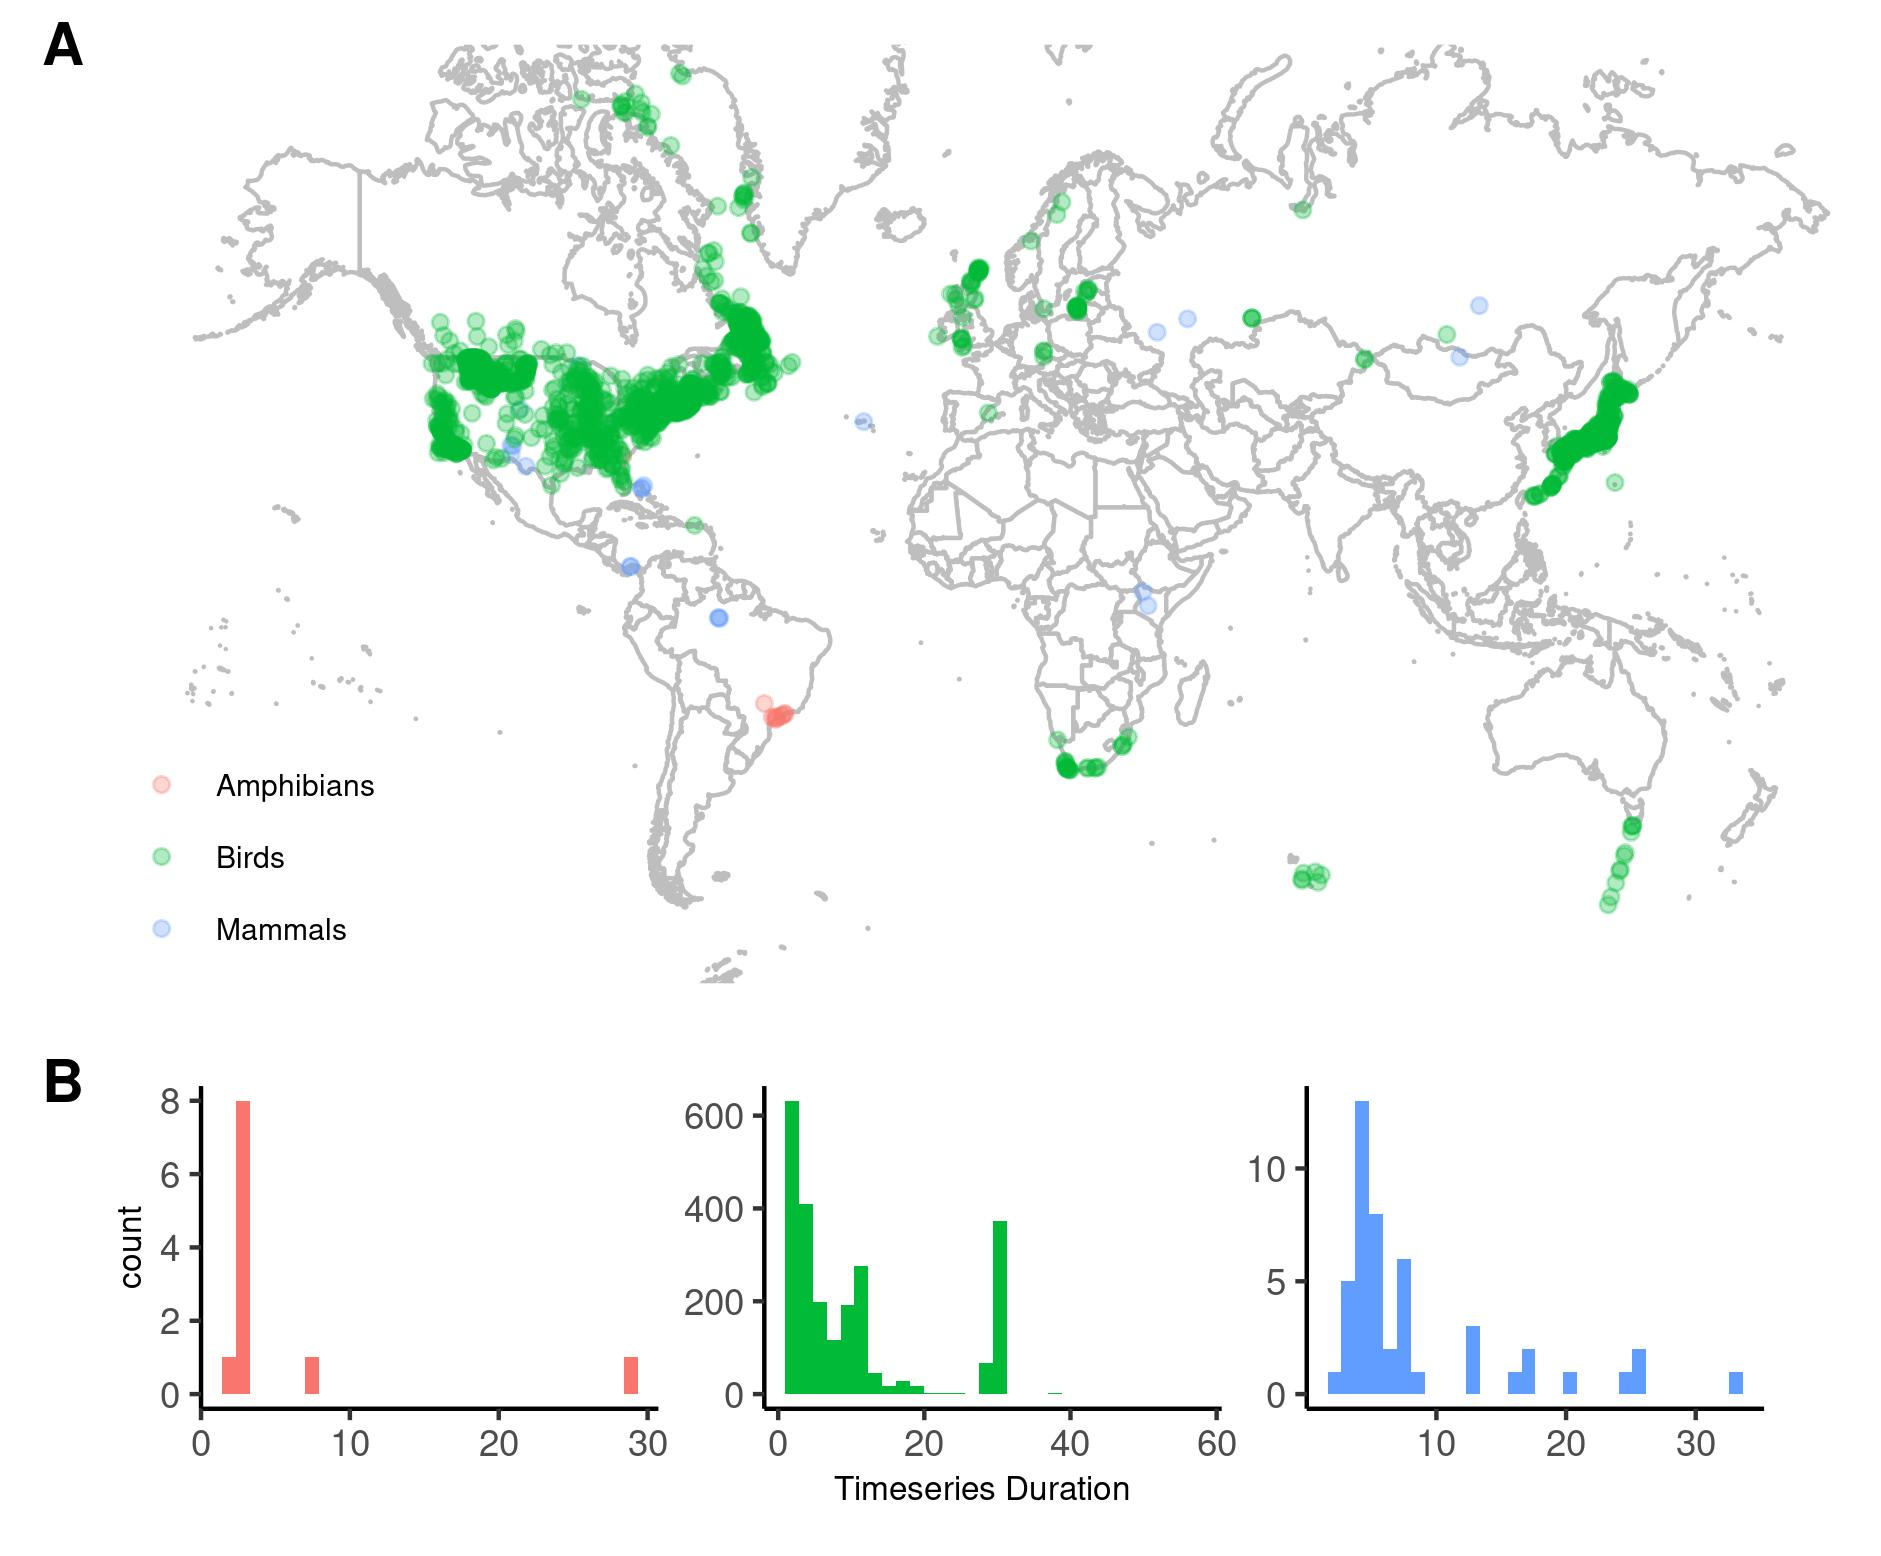
\includegraphics[width=\textwidth]{../../figures/study_map_hist} \caption{A) Map of time series locations with points colored by taxa, and B) histograms of time series duration broken down by taxa.}\label{fig:taxaMap}
\end{figure}

\hypertarget{diversity-metrics}{%
\subsection{Diversity Metrics}\label{diversity-metrics}}

We calculated yearly metrics of functional and species diversity for
each time series. Species-based metrics include species richness
(\emph{S}) and Jaccard similarity (\emph{J}) as a measure of turnover.
Jaccard similarity was calculated relative to the first observed year
for a time series. A negative trend in \emph{J} would therefore indicate
increasing turnover. We did not impose a correction for unobserved
species as non-parametric estimators do not assign species identities to
corrected richness values, and therefore could not be propagated to the
functional diversity metrics.

Functional diversity metrics were calculated using the \emph{dbFD}
function from the \emph{FD} R package (50). Here we report functional
richness (\emph{FRic}), functional evenness (\emph{FEve}), and
functional divergence (\emph{FDiv}) which together describe three
complementary characteristics of the functional space (22, 51).
\emph{FRic} assesses the volume of the trait space occupied by species
in the community, with higher values indicating communities with species
of more extreme trait values. \emph{FEve} describes how species are
distributed across the trait space and how abundance is distributed
across species. Higher values of \emph{FEve} indicate more even spacing
of species in the trait space and individuals across species.
\emph{FDiv} measures the degree to which species and their abundances
maximize differences in the functional space. Higher values of
\emph{FDiv} therefore correspond to communities where many highly
abundant species are on the edges of the trait space. We also calculated
the community-weighted mean (\emph{CWM}) of included traits to examine
shifts in the distribution of each trait.

All available trait data for each study were included in functional
diversity calculations with the exception of traits that were the same
value for all observed species in the study. For variables with multiple
levels each level was included as a separate trait axis. Continuous
traits were z-score scaled to give each trait equal weight in the trait
space (52, 53). The number of trait axes was limited to the maximum
number of traits that fulfills the criteria \(s >= 2^t\), where \(s\) is
the number of species and \emph{t} is the number of traits. This
restriction allows for enough axes to capture the trait space while
maintaining computational feasibility (54). Metrics incorporated
weighting based on species abundance.

\hypertarget{null-models}{%
\subsection{Null Models}\label{null-models}}

To assess functional change independent of species richness we
calculated the standardized effect size (SES) for each of the three
summary functional diversity metrics (\emph{FRic}, \emph{FEve},
\emph{FDiv}) from null estimates (55). Null model corrections allow us
to assess the degree to which the observed functional diversity metric
deviates from the value expected by chance in a randomly assembled
community. Null estimates were calculated for each rarefied sample by
randomly sampling species from the species pool for each year and
randomly assigning observed abundances to species. Species pools
included all species observed for a time series. This process was
repeated 500 times to get an estimate and standard deviation of the null
expectation for the metric for each rarefaction sample for that time
series. We used these values to calculate SES using the following
formula: \(SES = [F_{obs} - mean_{(F_{null})}]/SD_{(F_{null})}\). We
then calculated the median SES estimate for each metric from all the
rarefaction samples for a time series. SES estimates can be interpreted
as how much of the functional characteristic (richness, evenness,
divergence) was observed beyond what was expected by chance for a
community of that species richness.

\hypertarget{analysis}{%
\subsection{Analysis}\label{analysis}}

We estimated general trends for each diversity metric using a linear
mixed effects model with a random slope and intercept for each study and
each time series nested within the study. We fit 18 individual
\emph{CWM} models. All time series with data for a given trait were
included in the corresponding \emph{CWM} model. We estimated study level
trends using individual linear models. For studies with more than one
times series we fit a random slope and intercept for time series. Some
study-level models could not be fit for five studies for at least one
metric due to data limitations, but those studies were still included in
the general models. They represented 12 of 1350 study-level models fit
for each metric. For further details see the supplement. Where
appropriate, response variables were \(log\) or \(log(x+1)\) transformed
to better fit model assumptions of residual normality.

To test for trends within and between different levels of taxa, biome,
and realm we fit separate models with each of those factors added as a
predictor to the original model structure. We estimated within-level
slopes and calculated between-level contrasts using the \emph{emmeans}
package (v1.8.2, 56). We assessed the impact of time series duration and
start year on study-level trends using linear models with duration and
start year as predictors. All models in our analysis were fit using the
\emph{lme4} (v1.1-30) package in R (v4.2.3) and p-values were calculated
by Satterthwaite's degrees of freedom method using the \emph{lmerTest}
(v3.1-3) package with a significance level of \(\alpha = 0.05\)
(57--59).

\hypertarget{results}{%
\section{Results}\label{results}}

We found no significant overall trend in species richness or summary
functional diversity metrics (observed or standardized) (Fig
\ref{fig:timeseriesPlot}). We did find a significant overall decrease in
Jaccard similarity, indicating accumulating changes in species
composition. Non-significant overall trends indicate that although some
studies experience increasing or decreasing trends, the average trend
across studies was plausibly 0 (Table \ref{tab:resultsTab}). Trends for
different taxa, biomes, or realms were also non-significant for richness
and summary functional diversity metrics, with the exception of a
significantly increasing trend for functional evenness of global studies
(characterized by having samples on multiple continents), and a
significantly decreasing functional richness slope for
temperate/tropical studies and mammal studies. However, trends were not
exhibited for the standardized metric indicating that differences were
largely due to changes in species richness. Further, with only two
global studies, the trend should not be considered truly general. The
general trends for \emph{CWM} models were similarly not significant,
with a significant positive trend for only percentage of fish in diet
composition.

\begin{figure}
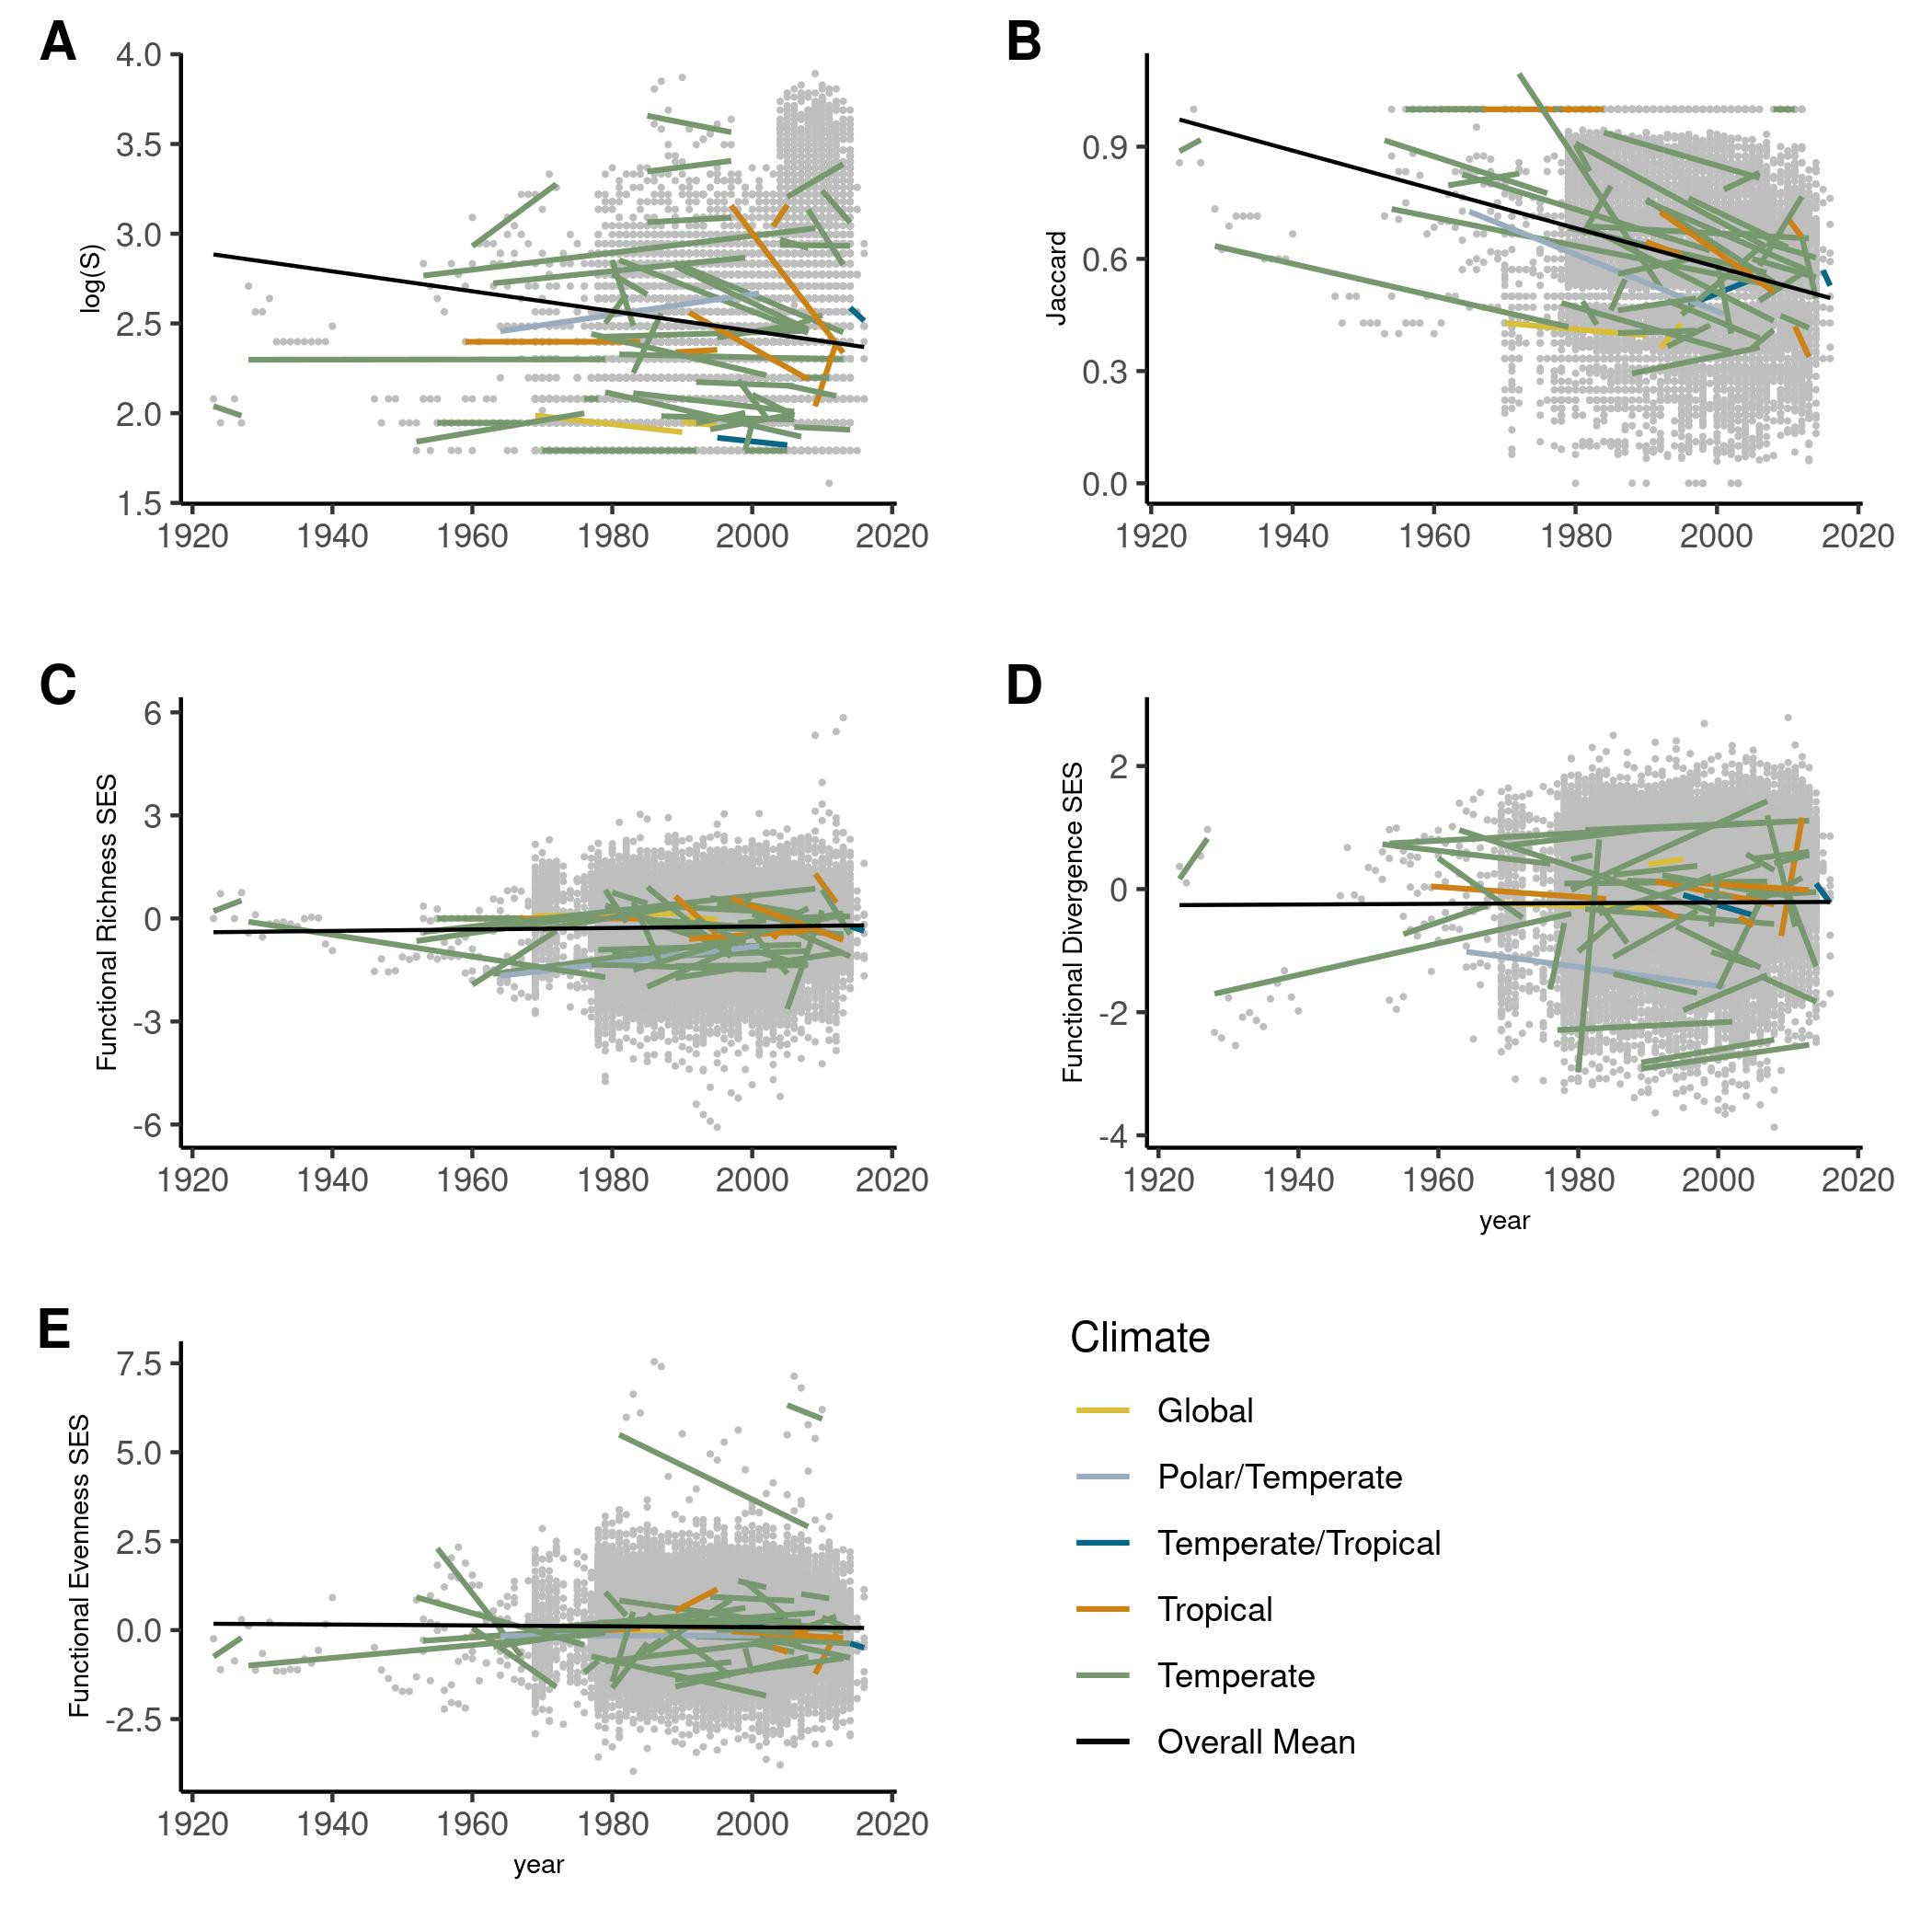
\includegraphics[width=\textwidth]{../../figures/3met_long} \caption{Plots of time series-level trends with line color corresponding to climatic region, with data points in grey and the overall metric mean in black for A) log species richness, B) Jaccard similarity, C) Functional Richness SES, D) Functional Divergence SES, and E) Functional Evenness SES}\label{fig:timeseriesPlot}
\end{figure}

\begin{table}[!h]

\caption{\label{tab:resultsTab}Model estimates and statistics for general trend models for species richness, Jaccard similarity, and standardized functional diversity metrics. Additional model estimates, including CWM models, can be found in the supplement.}
\centering
\resizebox{\linewidth}{!}{
\begin{tabular}[t]{l|l|>{\raggedright\arraybackslash}p{2cm}|l|r|r|l}
\hline
metric & effect & grouping & term & estimate & std.error & p.value\\
\hline
 &  &  & Intercept & -0.25 & 0.11 & 0.03\\
\cline{4-7}
 & \multirow{-2}{*}{\raggedright\arraybackslash fixed} & \multirow{-2}{2cm}{\raggedright\arraybackslash } & Year & 0.00 & 0.04 & 0.96\\
\cline{2-7}
 &  &  & SD Intercept & 0.60 &  & \\
\cline{4-7}
 &  &  & SD Year & 0.11 &  & \\
\cline{4-7}
 &  & \multirow{-3}{2cm}{\raggedright\arraybackslash study} & Corr(Intercept, Year) & -0.16 &  & \\
\cline{3-7}
 &  &  & SD Intercept & 0.60 &  & \\
\cline{4-7}
 &  &  & SD Year & 0.23 &  & \\
\cline{4-7}
\multirow{-8}{*}{\raggedright\arraybackslash SES\_FDiv} & \multirow{-6}{*}{\raggedright\arraybackslash random} & \multirow{-3}{2cm}{\raggedright\arraybackslash time series within study} & Corr(Intercept, Year) & -0.01 &  & \\
\cline{1-7}
 &  &  & Intercept & 0.09 & 0.16 & 0.59\\
\cline{4-7}
 & \multirow{-2}{*}{\raggedright\arraybackslash fixed} & \multirow{-2}{2cm}{\raggedright\arraybackslash } & Year & 0.00 & 0.01 & 0.73\\
\cline{2-7}
 &  &  & SD Intercept & 1.04 &  & \\
\cline{4-7}
 &  &  & SD Year & 0.02 &  & \\
\cline{4-7}
 &  & \multirow{-3}{2cm}{\raggedright\arraybackslash study} & Corr(Intercept, Year) & 1.00 &  & \\
\cline{3-7}
 &  &  & SD Intercept & 0.40 &  & \\
\cline{4-7}
 &  &  & SD Year & 0.17 &  & \\
\cline{4-7}
\multirow{-8}{*}{\raggedright\arraybackslash SES\_FEve} & \multirow{-6}{*}{\raggedright\arraybackslash random} & \multirow{-3}{2cm}{\raggedright\arraybackslash time series within study} & Corr(Intercept, Year) & -0.21 &  & \\
\cline{1-7}
 &  &  & Intercept & -0.26 & 0.07 & <0.001\\
\cline{4-7}
 & \multirow{-2}{*}{\raggedright\arraybackslash fixed} & \multirow{-2}{2cm}{\raggedright\arraybackslash } & Year & 0.04 & 0.04 & 0.35\\
\cline{2-7}
 &  &  & SD Intercept & 0.29 &  & \\
\cline{4-7}
 &  &  & SD Year & 0.11 &  & \\
\cline{4-7}
 &  & \multirow{-3}{2cm}{\raggedright\arraybackslash study} & Corr(Intercept, Year) & -0.27 &  & \\
\cline{3-7}
 &  &  & SD Intercept & 0.54 &  & \\
\cline{4-7}
 &  &  & SD Year & 0.18 &  & \\
\cline{4-7}
\multirow{-8}{*}{\raggedright\arraybackslash SES\_FRic} & \multirow{-6}{*}{\raggedright\arraybackslash random} & \multirow{-3}{2cm}{\raggedright\arraybackslash time series within study} & Corr(Intercept, Year) & 0.06 &  & \\
\cline{1-7}
 &  &  & Intercept & 0.46 & 0.02 & <0.001\\
\cline{4-7}
 & \multirow{-2}{*}{\raggedright\arraybackslash fixed} & \multirow{-2}{2cm}{\raggedright\arraybackslash } & Year & -0.03 & 0.01 & <0.001\\
\cline{2-7}
 &  &  & SD Intercept & 0.09 &  & \\
\cline{4-7}
 &  &  & SD Year & 0.02 &  & \\
\cline{4-7}
 &  & \multirow{-3}{2cm}{\raggedright\arraybackslash study} & Corr(Intercept, Year) & -0.35 &  & \\
\cline{3-7}
 &  &  & SD Intercept & 0.08 &  & \\
\cline{4-7}
 &  &  & SD Year & 0.02 &  & \\
\cline{4-7}
\multirow{-8}{*}{\raggedright\arraybackslash log(Jaccard + 1)} & \multirow{-6}{*}{\raggedright\arraybackslash random} & \multirow{-3}{2cm}{\raggedright\arraybackslash time series within study} & Corr(Intercept, Year) & 0.05 &  & \\
\cline{1-7}
 &  &  & Intercept & 2.40 & 0.10 & <0.001\\
\cline{4-7}
 & \multirow{-2}{*}{\raggedright\arraybackslash fixed} & \multirow{-2}{2cm}{\raggedright\arraybackslash } & Year & -0.06 & 0.05 & 0.17\\
\cline{2-7}
 &  &  & SD Intercept & 0.64 &  & \\
\cline{4-7}
 &  &  & SD Year & 0.27 &  & \\
\cline{4-7}
 &  & \multirow{-3}{2cm}{\raggedright\arraybackslash study} & Corr(Intercept, Year) & -0.70 &  & \\
\cline{3-7}
 &  &  & SD Intercept & 0.21 &  & \\
\cline{4-7}
 &  &  & SD Year & 0.09 &  & \\
\cline{4-7}
\multirow{-8}{*}{\raggedright\arraybackslash log(Species Richness)} & \multirow{-6}{*}{\raggedright\arraybackslash random} & \multirow{-3}{2cm}{\raggedright\arraybackslash time series within study} & Corr(Intercept, Year) & 0.34 &  & \\
\hline
\end{tabular}}
\end{table}

We did find significant differences between taxa, realms, and climate
for Jaccard similarity and some of the \emph{CWM's}. For example, while
Jaccard similarity was decreasing in the general trend and there were
significant within group slopes for Mammals, Birds, and Terrestrial
communities, there was no significant slope for the marine realm,
indicating that the general trend is mostly driven by turnover in
terrestrial communities. For bird communities, we also found within
group trends and between group differences for trends in foraging
behavior. We found a significant increasing trend in utilization of the
canopy in Tropical communities that was significantly different from the
trends for Polar/Temperate and Temperate communities. There was a
significant decrease in utilization of the understory for Terrestrial
communities and significant increase in foraging below the water surface
for global studies (but see the previous limitations of Global data).
There was also a significant positive slope for \emph{CWM} body mass for
the single Temperate/Tropical study (with three time series) which were
marine mammal communities.

We found significant dietary shifts across communities, with a
significant increase in fruit consumption in Terrestrial communities and
a significant decrease in nectar consumption in Tropical communities, a
trend significantly different than that for Terrestrial communities.
There was a significant increase in seed consumption in bird species,
which was significantly different from the trend for Mammal communities.
There was a significant increase in fish consumption for the two Global
studies. Vertebrate consumption significantly decreased for Marine
studies and for studies of Global and Tropical communities.

At the study level, 15 of 50 studies exhibited a significant trend in
species richness and 11 exhibited significant turnover. For observed
functional metrics, 25 of 50 studies exhibited a trend in a least one
metric, and 15 of 50 studies exhibited a significant trend for at least
one standardized metrics (Table \ref{tab:trendTab}). In general, there
were more significant trends for uncorrected metrics, with some
disappearing after correction, indicating that those trends were likely
due to changes in the number of species. Hypothesis testing for
study-level trends is likely affected by multiple testing issues and
some trends identified as significant are therefore potentially
spurious. Rather than interpreting changes in specific studies, we
present these results as a general picture of the kinds of trends
experienced by communities.

\begin{table}

\caption{\label{tab:trendTab}Number of studies that experienced a significant trend in each calculated metric out of 50 total studies.}
\centering
\begin{tabular}[t]{ccccccccc}
\toprule
 & S & Jaccard Similarity & FRic & FEve & FDiv & SES FRic & SES FEve & SES FDiv\\
\midrule
+ & 7 & 0 & 7 & 5 & 3 & 4 & 4 & 3\\
- & 8 & 11 & 8 & 6 & 5 & 2 & 6 & 2\\
\bottomrule
\end{tabular}
\end{table}

Study-level slopes for summary functional metrics were significantly
related to start year of the time series for Jaccard similarity and
functional evenness, both of which had significantly more negative
slopes with more recent start year. No summary functional metrics were
significantly related to the start year of the time series.

We assessed the sensitivity of general trend results to major data
processing decision by rerunning models with increasingly conservative
subsets of the data. After excluding time series with less than two,
three, and four year durations, we found that the general trend for
increase in CWM aerial foraging disappeared, but two other trends in
CWM's appeared. After excluding time series two years long, a general
trend appeared for increased CWM use of the forest canopy, and decreased
CWM of seed consumption. These two trends remained as increasingly
shorter time series were excluded suggesting the increase in aerial
foraging was an erroneous finding while the other two trends were more
robust. Percentage of species in a community with trait data did not
appear to have an affect on general trend results, as general trends
were unchanged with increasing cut offs for percentage of species with
trait data. A complete list of models run in the sensitivity analysis
and their results can be found in the supplement.

\hypertarget{discussion}{%
\section{Discussion}\label{discussion}}

Our study represents the largest broad-scale multi-taxa assessment of
functional change through time to date, giving a first look at aggregate
and local trends in functional diversity in mammal and bird communities.
Surprisingly, we did not detect an overall trend in any of the summary
functional diversity metrics. As with previous species-based syntheses,
we also found no overall trend in species richness accompanied by
increasing turnover through time (36), indicating that non-significant
trends in functional metrics may be consistent with similar
well-documented species derived trends. We found no trend in functional
change for almost all realms, biomes, and taxonomic groups, with
evidence of functional richness loss in mammal studies only. These
results are consistent with multiple studies linking anthropogenic
drivers to loss of functional diversity in mammal communities (60--62)

Despite a lack of general trends in summary functional metrics, we did
find multiple trends in \emph{CWM}'s for studies coming from the same
taxa, realms, or climates, many of which are consistent with previous
findings for those contexts. For example, the decrease in insect
consumption for tropical communities reflects well documented declines
in tropical insectivorous birds (63). Reduction in utilization of
understory foraging for terrestrial communities could be the result of
disturbance like human recreation or increased predation from introduced
species. Other shifts in diet for both Birds and Mammals, including
increasing fruit, seed, and vertebrate consumption and decreasing seed
consumption in some climates point to important areas for further
exploration.

At the study level, biodiversity change fell into four dominant
scenarios of change based on trends in richness, turnover, and
functional metrics: no change, only functional change, richness and
functional change with turnover, and richness and functional change
without turnover (Table \ref{tab:changeScenarios}). In contrast to our
expectation based on anthropogenic impacts, around a quarter of studies
experienced no trend in richness, turnover, or functional metrics. These
studies spanned the distribution of study durations excluding only the
very longest running studies, with the longest no change time series
lasting 23 years.

Another quarter of the studies showed no trend in richness or turnover,
but did show a significant shift in at least one summary functional
metric. These communities are best aligned with scenarios of species
replacement where only a few functional outliers replaced functionally
indistinct species or vice versa (there were studies with positive and
negative trends in all three functional metrics). Studies in the
scenario of only functional change were heavily skewed toward shorter
running time series, indicating that they may represent a limited
snapshot of communities that on longer time scales would be exhibiting
significant change in species-based metrics, particularly as species
replacement continued adding to turnover. Communities in this scenario,
and the previous scenario of no functional change are consistent with
hypotheses that species richness may be strongly regulated through time
(3, 8), and emphasize that maintenance of functional structure can be
divorced from those processes.

About 10 percent of studies, but the majority of time series in our
dataset, exhibited richness and functional change but no turnover. These
studies also spanned the the distribution of time series durations,
excluding the longest running studies. With the exception of one study,
trends in functional change for this group were only found for
uncorrected metrics and disappeared after correcting for species
richness, indicating that functional change in this group is almost
exclusively the result of species gains or losses rather than turnover
of species with different functional traits.

About 15 percent of studies, which were also exclusively the longest
running studies, had a trend in turnover, richness, and functional
change. The studies in this scenario fell into two groups: a positive
trend in richness with a positive trend in functional richness
(corrected and uncorrected), and a negative trend in species richness
with a negative trend in uncorrected functional richness and no trend in
corrected richness but a trend in other corrected functional metrics.
This would indicate that when species are lost from a community, they
are not more functionally unique than expected by chance, though they
may produce shifts in other aspects of functional structure. When
species are gained however, they disproportionately add to the
functional richness of the community.

Our results illustrate the range of relationships between species-based
and functional metrics observed in real communities. Critically,
particularly for the short observation time windows that characterize
the majority of ecological data, functional shifts may be underlying
seemingly static species-based community metrics. Species-based
approaches may therefore be missing areas where significant change in
the functional space could be impacting ecosystem function and
resilience. In scenarios where there are significant species gains or
losses over time, we found evidence that species losses may be
relatively functionally indistinct, while species gains contribute
disproportionately to the richness of a functional space. This finding
is consistent with evidence that at least in bird communities, common
functionally general species are being lost even as rare species are
increasing (64--66).

Our results are consistent with ecological expectations that community
dissimilarity would be greater the larger the observation time window
purely due to background processes, which is likely further accelerated
by global change drivers (14). While we do not address how observed
rates differ from background expectation here, we can make some
assertions about the implication of turnover for functional change.
Where turnover is occurring, it is almost always accompanied by a
directional change in the functional space. Species are not therefore
being replaced by exact functional counter parts. The fact that we
observed both increases and decreases in corrected functional richness
accompanying turnover is a reminder that replacements are not always an
indication of functional loss but can also lead to increased functional
richness. While shifts in functional space may be the result of
environmental pressure, we cannot distinguish between directional change
and shifts due to the inavailability of an analog species in the species
pool.

\begin{figure}
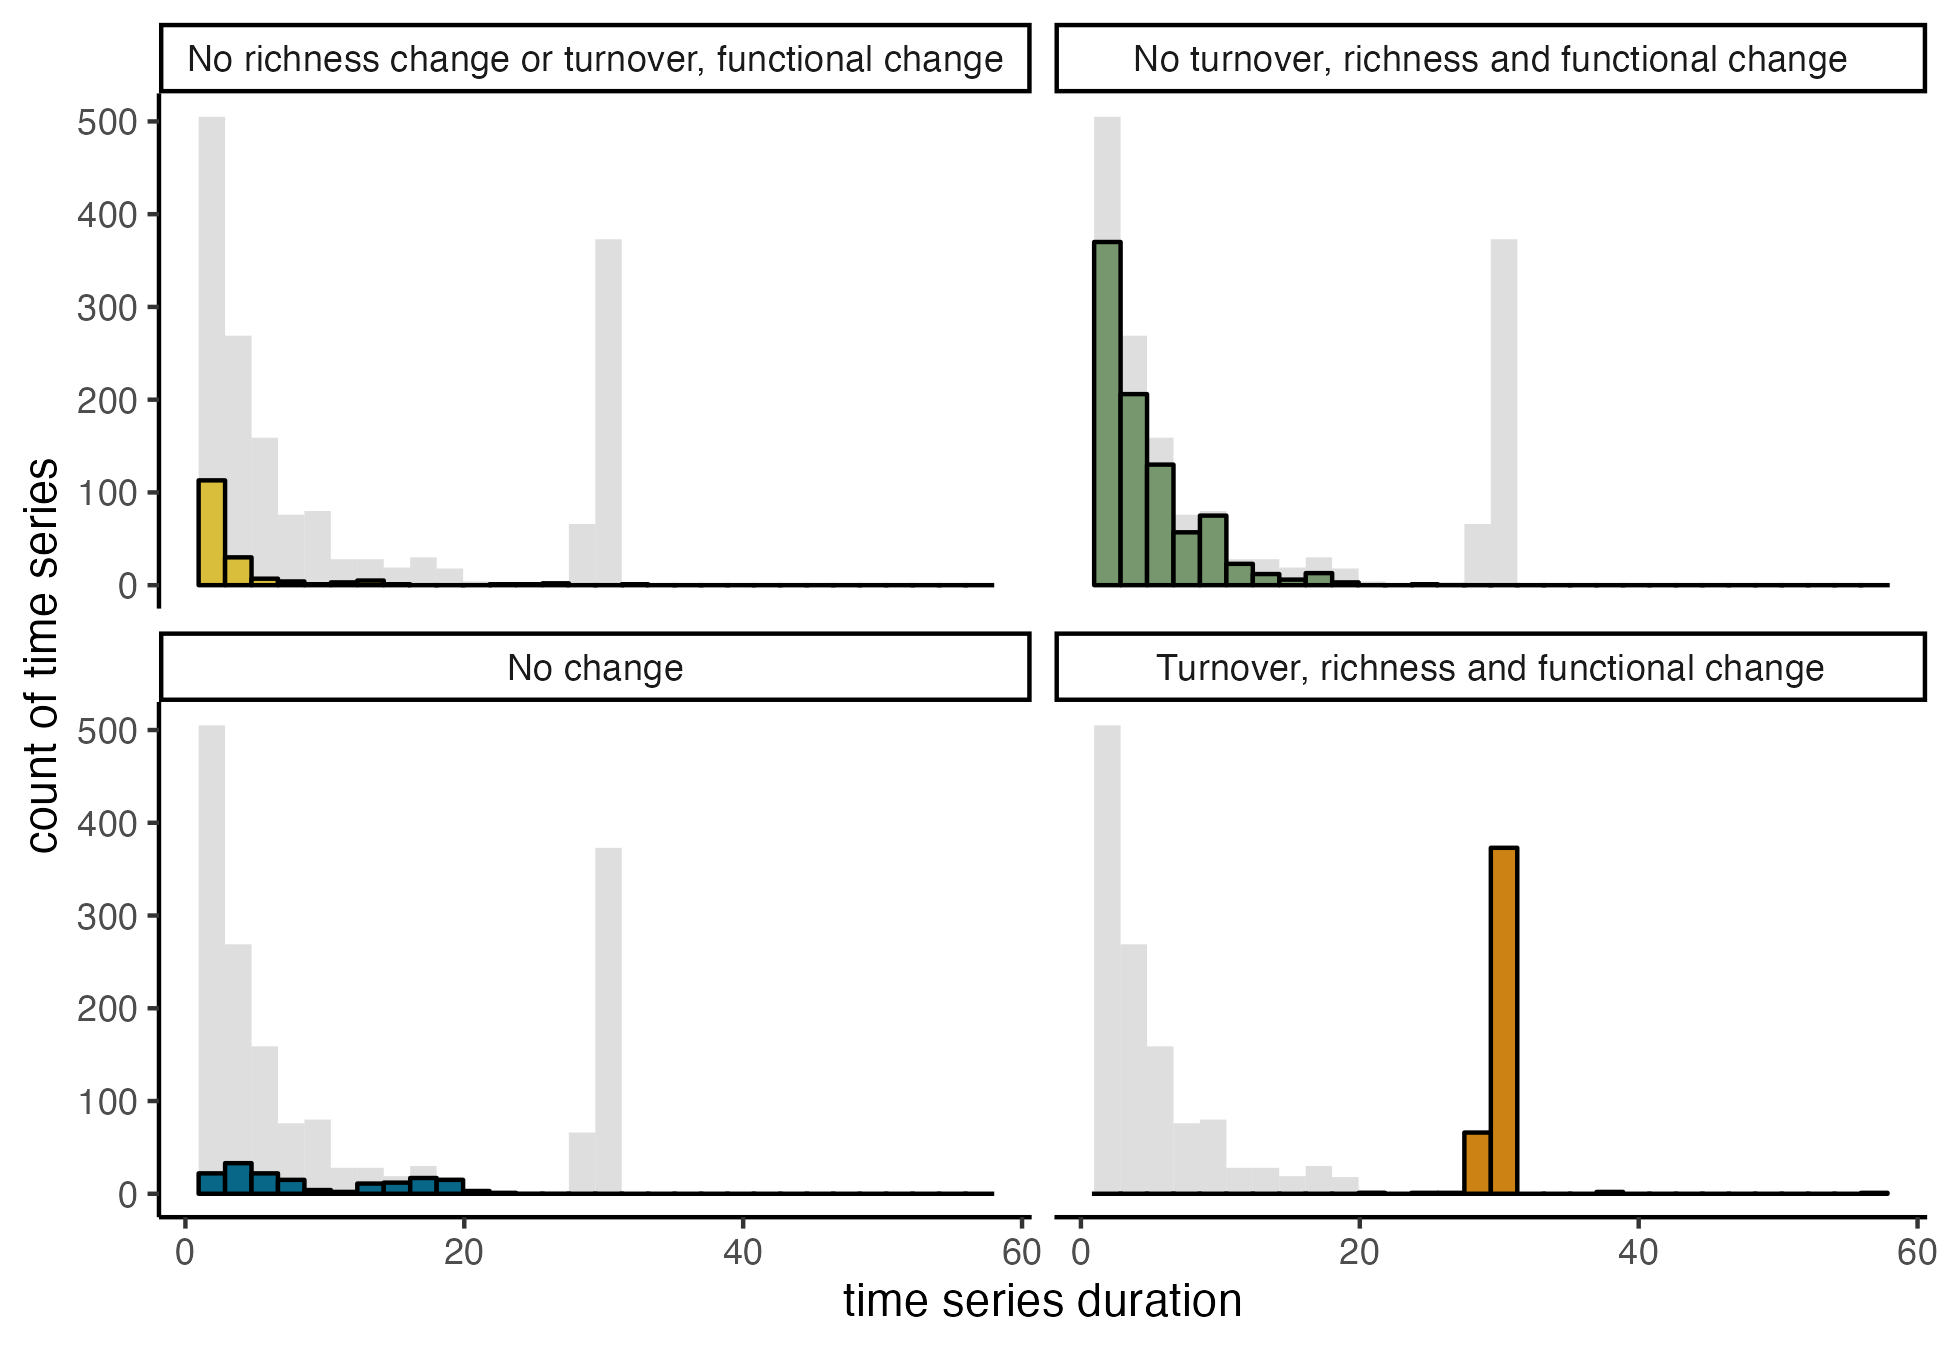
\includegraphics[width=\textwidth]{../../figures/duration_hist} 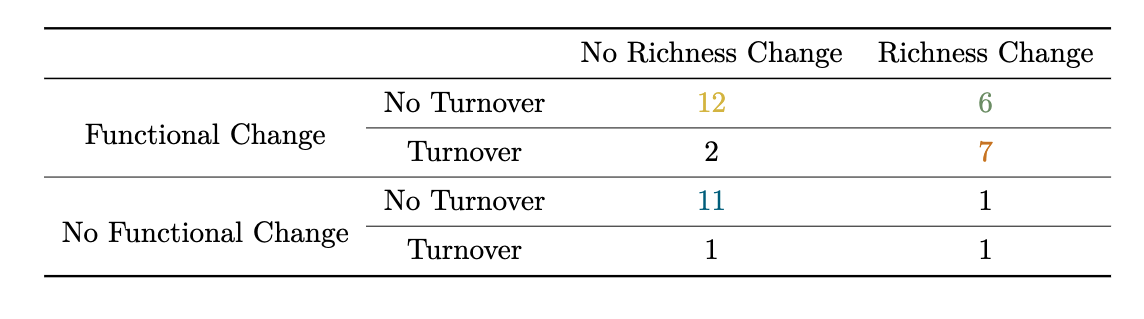
\includegraphics[width=\textwidth]{../../figures/functional_change_table} \caption{Comparision of the distribution of time series durations from each type of change to the overall distribution of time series durations, with no richness change or turnover and functional change in yellow, no turnover but richness and functional change in green, no change in blue, and turnover, richness and functional change studies in orange.}\label{fig:changeScenarios}
\end{figure}

Still, some results stand in contrast to predictions for trait shifts
under global change. For example, mean body size is predicted to
decrease as a result of climate change impacts and megafaunal loss (67),
a phenomenon which has already been well documented empirically and
experimentally in multiple taxa (68--71). While the species-level trait
means used here are not appropriate for assessing intraspecific body
size shifts, we would expect to see shifts in community-wide means due
to local losses of large-bodied species. Instead, we found no evidence
of a trend in \emph{CWM} body size, with the exception of a single study
of marine mammals in the Bahamas which showed a significant increase.
Still, many of the studies in our dataset draw from areas that may have
experienced significant loss of large-bodied species before the
observation window, with contemporary loss rates slowing (72). Trends
could be significantly different for the same time periods in regions of
sub-Saharan Africa, for example, which has poor representation in our
dataset but where megafauna exist on the landscape and are increasingly
threatened (73).

What does local maintenance of functional structure mean for ecosystem
function? The vast majority of experimental and observational work links
declines in function to declines in functional or species diversity (7,
18, 74). By those criteria very few communities in our dataset are in a
state of concern for loss of functionality (Table \ref{tab:trendTab}),
though we did find evidence that mammal communities may be in greater
danger than bird communities. Still, shifts in metrics are only relevant
if the underlying traits are those most critical for ecosystem function.
We were limited in this analysis to the traits available rather than
those with strong empirical links to function. Similarly, the dimensions
of functional space most important for ecosystem function are still a
topic of on going debate, and at least some known aspects important for
multifunctionality were not measured here (e.g.~dispersion, rarity,
abundance of dominant species, 75).

\hypertarget{potential-methodological-limitations}{%
\subsection{Potential Methodological
Limitations}\label{potential-methodological-limitations}}

Here we approach the question of functional change using the best
available data and biodiversity synthesis approaches. While we found
signatures of change at the study level, some gaps in best practices may
be obscuring a true general trend at the aggregate level. First, the
BioTIME database, while the most comprehensive data source of time
series available, is limited in temporal and geographic scope. Most time
series span only a few years (Fig \ref{fig:taxaMap}) and may not provide
the statistical power necessary to detect trends (76). The database is
also not a representative sample of the world's biodiversity or areas of
greatest threat (6, 12), and the subset of data in this study is
predominantly from North America. We may simply not have data from those
areas experiencing the greatest perturbation (77), particularly
scenarios of conversion to urban, human-dominated landscapes. While
evidence from other work shows even disturbed communities can maintain
functional structure (32, 34), these results should not be interpreted
as evidence of low functional impact in areas of heavy human
disturbance.

Second, despite using the most comprehensive trait databases for these
taxa, we were still limited to species-level means of the traits deemed
important by database creators. The importance of intraspecific
variation is well documented (78, 79), however individual-level traits
are rarely collected alongside monitoring data, especially for the
longest running efforts. Species-level traits may be obscuring more
subtle shifts in the trait space happening within species. Likewise,
available trait data may not capture the traits experiencing the
greatest change. For example, we focus here mostly on ecological traits
(i.e.~foraging strategy, diet, etc) rather than life-history or
reproductive traits.

Third, while we use here the most common metrics for describing
functional diversity, they do not measure some potentially important
aspects of the functional space. Most notably, the summary metrics we
calculated do not capture shifts in the location of the functional space
as a whole. For example, two communities could have very similar metric
values but no overlap in their trait spaces. This is especially relevant
in the context of biodiversity change as a species loss could be
replaced by a species with very different functional attributes, but the
replacement would go undetected if the new species expanded the trait
space by the same degree and had similar abundance. This scenario may be
common in communities tracking changing environmental conditions. While
trait CWM's capture axis shifts, approaches for assessing
multidimensional shifts in functional space are still relatively new
(54, 80, 81) but could shed critical insight into functional composition
changes of this nature.

\hypertarget{policy-implications}{%
\subsection{Policy Implications}\label{policy-implications}}

While we found no over all trends in functional metrics, our results
should not be interpreted as an indication that the ongoing biodiversity
crisis is less severe than previously described, or that there is no
concern for functional change as a result of anthropogenic impact. In
fact, study-level trends indicate quite the opposite, that functional
shifts with unknown implications for ecosystem processes may be going
undetected by common species-based approaches, particularly for short
observation time windows. While the majority of studies in our dataset
did not experience a significant functional loss, a substantial body of
work links functional degradation to species losses as a result of
direct human intervention in the form of land use change and
intensification or habitat fragmentation, indicating that those studies
are simply not representative of the kinds of impacts of greatest policy
concern (31, 82, 83).

\hypertarget{future-work}{%
\subsection{Future Work}\label{future-work}}

We present here four prevailing scenarios of change experienced in bird
and mammal communities. While we offer a first discussion of which kinds
of change are most common and why, assessing the true global prevalence
will require continued efforts to fill data gaps, a well recognized
challenge in ecology (6, 12, 77). Still, a ``scenarios of change''
framework can provide structure for future work addressing functional
shifts, particularly as we reconcile results from broad-scale syntheses
with in-depth single system studies. It will be particularly critical to
link forms of change to individual drivers to assess which drivers may
impact species and functional diversity differently. Understanding those
links will help identify where directly measuring functional structure
instead of just species change is necessary for understand impacts on a
given system. In addition, direct links to drivers will improve our
ability to distinguish between communities experiencing no change due to
a lack of perturbation from communities with high resilience in the face
of disturbance.

Here we identify trends that are statistically significant, however they
may not necessarily be ecologically significant. While it is common to
link changes in functional metrics to changes in ecosystem processes,
those changes are less frequently discussed in terms of the size
necessary for ecological impact. The degree of change in a process
considered ecological meaningful is somewhat subjective and a function
of the system and management context, making identifying the ecological
meaning of broad-scale aggregate shifts even more challenging. It is
further hampered by the use of species-level trait data, as the traits
most closely linked to a process of interest may not be available (84).
Future trait collection that explicitly considers existing frameworks
for linking traits to processes (e.g.~the response and effect framework
15) would facilitate improved ecological interpretation of potential
functional changes.

\hypertarget{acknowledgments}{%
\section{Acknowledgments}\label{acknowledgments}}

We thank the scientists who contributed to and maintain the biodiversity
databases included in this study, including BioTIME, Amphibio, and Elton
Traits.

We thank Dr Shane Blowes and Dr Sarah Supp, whose code we adapted for
initial data processing of the BioTIME database.

\hypertarget{references}{%
\section*{References}\label{references}}
\addcontentsline{toc}{section}{References}

\hypertarget{refs}{}
\begin{CSLReferences}{0}{0}
\leavevmode\vadjust pre{\hypertarget{ref-barnosky2011}{}}%
\CSLLeftMargin{1. }%
\CSLRightInline{Barnosky AD, et al. (2011)
\href{https://doi.org/10.1038/nature09678}{Has the Earth{'}s sixth mass
extinction already arrived?} \emph{Nature} 471(7336):51--57.}

\leavevmode\vadjust pre{\hypertarget{ref-sully2019}{}}%
\CSLLeftMargin{2. }%
\CSLRightInline{Sully S, Burkepile DE, Donovan MK, Hodgson G, van Woesik
R (2019) \href{https://doi.org/10.1038/s41467-019-09238-2}{A global
analysis of coral bleaching over the past two decades}. \emph{Nature
Communications} 10(1):1264.}

\leavevmode\vadjust pre{\hypertarget{ref-brown2001}{}}%
\CSLLeftMargin{3. }%
\CSLRightInline{Brown JH, Ernest SKM, Parody JM, Haskell JP (2001)
\href{http://www.jstor.org/stable/4222853}{Regulation of diversity:
Maintenance of species richness in changing environments}.
\emph{Oecologia} 126(3):321--332.}

\leavevmode\vadjust pre{\hypertarget{ref-dornelas2014}{}}%
\CSLLeftMargin{4. }%
\CSLRightInline{Dornelas M, et al. (2014)
\href{https://doi.org/10.1126/science.1248484}{Assemblage Time Series
Reveal Biodiversity Change but Not Systematic Loss}. \emph{Science}
344(6181):296--299.}

\leavevmode\vadjust pre{\hypertarget{ref-vellend2013}{}}%
\CSLLeftMargin{5. }%
\CSLRightInline{Vellend M, et al. (2013)
\href{https://doi.org/10.1073/pnas.1312779110}{Global meta-analysis
reveals no net change in local-scale plant biodiversity over time}.
\emph{Proceedings of the National Academy of Sciences}
110(48):19456--19459.}

\leavevmode\vadjust pre{\hypertarget{ref-vellend2017}{}}%
\CSLLeftMargin{6. }%
\CSLRightInline{Vellend M, et al. (2017)
\href{https://doi.org/10.1002/ecy.1660}{Estimates of local biodiversity
change over time stand up to scrutiny}. \emph{Ecology} 98(2):583--590.}

\leavevmode\vadjust pre{\hypertarget{ref-brose2016}{}}%
\CSLLeftMargin{7. }%
\CSLRightInline{Brose U, Hillebrand H (2016)
\href{https://doi.org/10.1098/rstb.2015.0267}{Biodiversity and ecosystem
functioning in dynamic landscapes}. \emph{Philosophical Transactions of
the Royal Society B: Biological Sciences} 371(1694):20150267.}

\leavevmode\vadjust pre{\hypertarget{ref-gotelli2017}{}}%
\CSLLeftMargin{8. }%
\CSLRightInline{Gotelli NJ, et al. (2017) Community-level regulation of
temporal trends in biodiversity. \emph{Science Advances} 3(7).
doi:\href{https://doi.org/10.1126/sciadv.1700315}{10.1126/sciadv.1700315}.}

\leavevmode\vadjust pre{\hypertarget{ref-li2020}{}}%
\CSLLeftMargin{9. }%
\CSLRightInline{Li D, et al. (2020)
\href{https://doi.org/10.1098/rspb.2020.0777}{Changes in taxonomic and
phylogenetic diversity in the anthropocene}. \emph{Proceedings of the
Royal Society B: Biological Sciences} 287(1929):20200777.}

\leavevmode\vadjust pre{\hypertarget{ref-cardinale2014}{}}%
\CSLLeftMargin{10. }%
\CSLRightInline{Cardinale B (2014)
\href{https://doi.org/10.1126/science.344.6188.1098-a}{Overlooked local
biodiversity loss}. \emph{Science} 344(6188):1098--1098.}

\leavevmode\vadjust pre{\hypertarget{ref-cardinale2018}{}}%
\CSLLeftMargin{11. }%
\CSLRightInline{Cardinale BJ, Gonzalez A, Allington GRH, Loreau M (2018)
Is local biodiversity declining or not? A summary of the debate over
analysis of species richness time trends. \emph{Biological
Conservation}.
doi:\href{https://doi.org/10.1016/j.biocon.2017.12.021}{10.1016/j.biocon.2017.12.021}.}

\leavevmode\vadjust pre{\hypertarget{ref-gonzalez2016}{}}%
\CSLLeftMargin{12. }%
\CSLRightInline{Gonzalez A, et al. (2016)
\href{https://doi.org/10.1890/15-1759.1}{Estimating local biodiversity
change: a critique of papers claiming no net loss of local diversity}.
\emph{Ecology} 97(8):1949--1960.}

\leavevmode\vadjust pre{\hypertarget{ref-primack2018}{}}%
\CSLLeftMargin{13. }%
\CSLRightInline{Primack RB, et al. (2018)
\href{https://doi.org/10.1016/j.biocon.2017.12.023}{Biodiversity gains?
The debate on changes in local- vs global-scale species richness}.
\emph{Biological Conservation} 219:A1--A3.}

\leavevmode\vadjust pre{\hypertarget{ref-dornelas2023}{}}%
\CSLLeftMargin{14. }%
\CSLRightInline{Dornelas M, et al. (2023)
\href{https://doi.org/10.1098/rstb.2022.0199}{Looking back on
biodiversity change: Lessons for the road ahead}. \emph{Philosophical
Transactions of the Royal Society B: Biological Sciences}
378(1881):20220199.}

\leavevmode\vadjust pre{\hypertarget{ref-lavorel2002}{}}%
\CSLLeftMargin{15. }%
\CSLRightInline{Lavorel S, Garnier E (2002)
\href{https://doi.org/10.1046/j.1365-2435.2002.00664.x}{Predicting
changes in community composition and ecosystem functioning from plant
traits: revisiting the Holy Grail}. \emph{Functional Ecology}
16(5):545--556.}

\leavevmode\vadjust pre{\hypertarget{ref-mcgill2006}{}}%
\CSLLeftMargin{16. }%
\CSLRightInline{Mcgill B, Enquist B, Weiher E, Westoby M (2006)
\href{https://doi.org/10.1016/j.tree.2006.02.002}{Rebuilding community
ecology from functional traits}. \emph{Trends in Ecology \& Evolution}
21(4):178--185.}

\leavevmode\vadjust pre{\hypertarget{ref-suding2008}{}}%
\CSLLeftMargin{17. }%
\CSLRightInline{Suding KN, et al. (2008)
\href{https://doi.org/10.1111/j.1365-2486.2008.01557.x}{Scaling
environmental change through the community-level: a trait-based
response-and-effect framework for plants}. \emph{Global Change Biology}
14(5):1125--1140.}

\leavevmode\vadjust pre{\hypertarget{ref-cadotte2011}{}}%
\CSLLeftMargin{18. }%
\CSLRightInline{Cadotte MW, Carscadden K, Mirotchnick N (2011)
\href{https://doi.org/10.1111/j.1365-2664.2011.02048.x}{Beyond species:
functional diversity and the maintenance of ecological processes and
services}. \emph{Journal of Applied Ecology} 48(5):1079--1087.}

\leavevmode\vadjust pre{\hypertarget{ref-gagic2015}{}}%
\CSLLeftMargin{19. }%
\CSLRightInline{Gagic V, et al. (2015)
\href{https://doi.org/10.1098/rspb.2014.2620}{Functional identity and
diversity of animals predict ecosystem functioning better than
species-based indices}. \emph{Proceedings of the Royal Society B:
Biological Sciences} 282(1801):20142620.}

\leavevmode\vadjust pre{\hypertarget{ref-craven2018}{}}%
\CSLLeftMargin{20. }%
\CSLRightInline{Craven D, et al. (2018)
\href{https://doi.org/10.1038/s41559-018-0647-7}{Multiple facets of
biodiversity drive the diversity{\textendash}stability relationship}.
\emph{Nature Ecology \& Evolution}:1.}

\leavevmode\vadjust pre{\hypertarget{ref-morin2014}{}}%
\CSLLeftMargin{21. }%
\CSLRightInline{Morin X, Fahse L, Mazancourt C de, Scherer-Lorenzen M,
Bugmann H (2014) \href{https://doi.org/10.1111/ele.12357}{Temporal
stability in forest productivity increases with tree diversity due to
asynchrony in species dynamics}. \emph{Ecology Letters}
17(12):1526--1535.}

\leavevmode\vadjust pre{\hypertarget{ref-hillebrand2009}{}}%
\CSLLeftMargin{22. }%
\CSLRightInline{Hillebrand H, Matthiessen B (2009)
\href{https://doi.org/10.1111/j.1461-0248.2009.01388.x}{Biodiversity in
a complex world: consolidation and progress in functional biodiversity
research: Consolidation and progress in BDEF research}. \emph{Ecology
Letters} 12(12):1405--1419.}

\leavevmode\vadjust pre{\hypertarget{ref-cardinale2012}{}}%
\CSLLeftMargin{23. }%
\CSLRightInline{Cardinale BJ, et al. (2012)
\href{https://doi.org/10.1038/nature11148}{Biodiversity loss and its
impact on humanity}. \emph{Nature} 486(7401):59--67.}

\leavevmode\vadjust pre{\hypertarget{ref-dirzo2014}{}}%
\CSLLeftMargin{24. }%
\CSLRightInline{Dirzo R, et al. (2014)
\href{https://doi.org/10.1126/science.1251817}{Defaunation in the
Anthropocene}. \emph{Science} 345(6195):401--406.}

\leavevmode\vadjust pre{\hypertarget{ref-young2016}{}}%
\CSLLeftMargin{25. }%
\CSLRightInline{Young HS, McCauley DJ, Galetti M, Dirzo R (2016)
\href{https://doi.org/10.1146/annurev-ecolsys-112414-054142}{Patterns,
causes, and consequences of anthropocene defaunation}. \emph{Annual
Review of Ecology, Evolution, and Systematics} 47(1):333--358.}

\leavevmode\vadjust pre{\hypertarget{ref-daz2001}{}}%
\CSLLeftMargin{26. }%
\CSLRightInline{Dıáz S, Cabido M (2001)
\href{https://doi.org/10.1016/S0169-5347(01)02283-2}{Vive la différence:
Plant functional diversity matters to ecosystem processes}. \emph{Trends
in Ecology \& Evolution} 16(11):646--655.}

\leavevmode\vadjust pre{\hypertarget{ref-petchey2009}{}}%
\CSLLeftMargin{27. }%
\CSLRightInline{Petchey OL, Gaston KJ (2009)
\href{https://doi.org/10.1007/s12080-009-0041-9}{Effects on ecosystem
resilience of biodiversity, extinctions, and the structure of regional
species pools}. \emph{Theoretical Ecology} 2(3):177--187.}

\leavevmode\vadjust pre{\hypertarget{ref-gallagher2013}{}}%
\CSLLeftMargin{28. }%
\CSLRightInline{Gallagher RV, Hughes L, Leishman MR (2013)
\href{https://doi.org/10.1111/j.1600-0587.2012.07514.x}{Species loss and
gain in communities under future climate change: consequences for
functional diversity}. \emph{Ecography} 36(5):531--540.}

\leavevmode\vadjust pre{\hypertarget{ref-petchey2002}{}}%
\CSLLeftMargin{29. }%
\CSLRightInline{Petchey OL, Gaston KJ (2002)
\href{https://doi.org/10.1098/rspb.2002.2073}{Extinction and the loss of
functional diversity}. \emph{Proceedings of the Royal Society of London
Series B: Biological Sciences} 269(1501):1721--1727.}

\leavevmode\vadjust pre{\hypertarget{ref-pimiento2020}{}}%
\CSLLeftMargin{30. }%
\CSLRightInline{Pimiento C, et al. (2020)
\href{https://doi.org/10.1126/sciadv.aay7650}{Functional diversity of
marine megafauna in the Anthropocene}. \emph{Science Advances}
6(16):eaay7650.}

\leavevmode\vadjust pre{\hypertarget{ref-flynn2009}{}}%
\CSLLeftMargin{31. }%
\CSLRightInline{Flynn DFB, et al. (2009)
\href{https://doi.org/10.1111/j.1461-0248.2008.01255.x}{Loss of
functional diversity under land use intensification across multiple
taxa}. \emph{Ecology Letters} 12(1):22--33.}

\leavevmode\vadjust pre{\hypertarget{ref-edwards2013}{}}%
\CSLLeftMargin{32. }%
\CSLRightInline{Edwards FA, Edwards DP, Hamer KC, Davies RG (2013)
\href{https://doi.org/10.1111/ibi.12027}{Impacts of logging and
conversion of rainforest to oil palm on the functional diversity of
birds in Sundaland}. \emph{Ibis} 155(2):313--326.}

\leavevmode\vadjust pre{\hypertarget{ref-larsen2018}{}}%
\CSLLeftMargin{33. }%
\CSLRightInline{Larsen S, Chase JM, Durance I, Ormerod SJ (2018)
\href{https://doi.org/10.1002/ecy.2213}{Lifting the veil: richness
measurements fail to detect systematic biodiversity change over three
decades}. \emph{Ecology} 99(6):1316--1326.}

\leavevmode\vadjust pre{\hypertarget{ref-matuoka2020}{}}%
\CSLLeftMargin{34. }%
\CSLRightInline{Matuoka MA, Benchimol M, Almeida-Rocha JM de,
Morante-Filho JC (2020)
\href{https://doi.org/10.1016/j.ecolind.2020.106471}{Effects of
anthropogenic disturbances on bird functional diversity: A global
meta-analysis}. \emph{Ecological Indicators} 116:106471.}

\leavevmode\vadjust pre{\hypertarget{ref-jackson2015}{}}%
\CSLLeftMargin{35. }%
\CSLRightInline{Jackson ST, Blois JL (2015)
\href{https://doi.org/10.1073/pnas.1403664111}{Community ecology in a
changing environment: Perspectives from the Quaternary}.
\emph{Proceedings of the National Academy of Sciences}
112(16):4915--4921.}

\leavevmode\vadjust pre{\hypertarget{ref-dornelas2018}{}}%
\CSLLeftMargin{36. }%
\CSLRightInline{Dornelas M, et al. (2018)
\href{https://doi.org/10.1111/geb.12729}{BioTIME: A database of
biodiversity time series for the Anthropocene}. \emph{Global Ecology and
Biogeography} 27(7):760--786.}

\leavevmode\vadjust pre{\hypertarget{ref-pimiento2017}{}}%
\CSLLeftMargin{37. }%
\CSLRightInline{Pimiento C, et al. (2017)
\href{https://doi.org/10.1038/s41559-017-0223-6}{The Pliocene marine
megafauna extinction and its impact on functional diversity}.
\emph{Nature Ecology \& Evolution} 1(8):1100--1106.}

\leavevmode\vadjust pre{\hypertarget{ref-hedberg2022}{}}%
\CSLLeftMargin{38. }%
\CSLRightInline{Hedberg CP, Lyons SK, Smith FA (2022)
\href{https://doi.org/10.1111/geb.13428}{The hidden legacy of megafaunal
extinction: Loss of functional diversity and resilience over the Late
Quaternary at Hall{'}s Cave}. \emph{Global Ecology and Biogeography}
31(2):294--307.}

\leavevmode\vadjust pre{\hypertarget{ref-estes2011}{}}%
\CSLLeftMargin{39. }%
\CSLRightInline{Estes JA, et al. (2011)
\href{https://doi.org/10.1126/science.1205106}{Trophic Downgrading of
Planet Earth}. \emph{Science} 333(6040):301--306.}

\leavevmode\vadjust pre{\hypertarget{ref-smith2018}{}}%
\CSLLeftMargin{40. }%
\CSLRightInline{Smith FA, Elliott Smith RE, Lyons SK, Payne JL (2018)
\href{https://doi.org/10.1126/science.aao5987}{Body size downgrading of
mammals over the late quaternary}. \emph{Science} 360(6386):310--313.}

\leavevmode\vadjust pre{\hypertarget{ref-trindade-santos2020}{}}%
\CSLLeftMargin{41. }%
\CSLRightInline{Trindade-Santos I, Moyes F, Magurran AE (2020)
\href{https://doi.org/10.1098/rspb.2020.0889}{Global change in the
functional diversity of marine fisheries exploitation over the past 65
years}. \emph{Proceedings of the Royal Society B: Biological Sciences}
287(1933):20200889.}

\leavevmode\vadjust pre{\hypertarget{ref-jarzyna2016}{}}%
\CSLLeftMargin{42. }%
\CSLRightInline{Jarzyna MA, Jetz W (2016)
\href{https://doi.org/10.1111/gcb.13571}{A near half-century of temporal
change in different facets of avian diversity}. \emph{Global Change
Biology} 23(8):2999--3011.}

\leavevmode\vadjust pre{\hypertarget{ref-barnagaud2017}{}}%
\CSLLeftMargin{43. }%
\CSLRightInline{Barnagaud J-Y, Gaüzère P, Zuckerberg B, Princé K,
Svenning J-C (2017)
\href{https://doi.org/10.1007/s00442-017-3967-4}{Temporal changes in
bird functional diversity across the United States}. \emph{Oecologia}
185(4):737--748.}

\leavevmode\vadjust pre{\hypertarget{ref-duxedaz2022}{}}%
\CSLLeftMargin{44. }%
\CSLRightInline{Díaz S, Malhi Y (2022)
\href{https://doi.org/10.1146/annurev-environ-120120-054300}{Biodiversity:
Concepts, patterns, trends, and perspectives}. \emph{Annual Review of
Environment and Resources} 47(1):31--63.}

\leavevmode\vadjust pre{\hypertarget{ref-fitzjohn2014}{}}%
\CSLLeftMargin{45. }%
\CSLRightInline{FitzJohn RG, et al. (2014)
\href{https://doi.org/10.1111/1365-2745.12260}{How much of the world is
woody?} \emph{Journal of Ecology} 102(5):1266--1272.}

\leavevmode\vadjust pre{\hypertarget{ref-wilman2014}{}}%
\CSLLeftMargin{46. }%
\CSLRightInline{Wilman H, et al. (2014)
\href{https://doi.org/10.1890/13-1917.1}{EltonTraits 1.0: Species-level
foraging attributes of the world's birds and mammals: {\emph{Ecological
Archives}} E095-178}. \emph{Ecology} 95(7):2027--2027.}

\leavevmode\vadjust pre{\hypertarget{ref-blowes2019}{}}%
\CSLLeftMargin{47. }%
\CSLRightInline{Blowes SA, et al. (2019)
\href{https://doi.org/10.1126/science.aaw1620}{The geography of
biodiversity change in marine and terrestrial assemblages}.
\emph{Science} 366(6463):339--345.}

\leavevmode\vadjust pre{\hypertarget{ref-norman2020}{}}%
\CSLLeftMargin{48. }%
\CSLRightInline{Norman KEA, Chamberlain S, Boettiger C (2020)
\href{https://doi.org/10.1111/2041-210X.13440}{taxadb: A
high-performance local taxonomic database interface}. \emph{Methods in
Ecology and Evolution} 11(9):1153--1159.}

\leavevmode\vadjust pre{\hypertarget{ref-rcoreteam2021}{}}%
\CSLLeftMargin{49. }%
\CSLRightInline{R Core Team (2021) \emph{R: A language and environment
for statistical computing} (R Foundation for Statistical Computing,
Vienna, Austria) Available at: \url{https://www.R-project.org/}.}

\leavevmode\vadjust pre{\hypertarget{ref-lalibertuxe92010}{}}%
\CSLLeftMargin{50. }%
\CSLRightInline{Laliberté E, Legendre P (2010)
\href{https://doi.org/10.1890/08-2244.1}{A distance-based framework for
measuring functional diversity from multiple traits}. \emph{Ecology}
91(1):299--305.}

\leavevmode\vadjust pre{\hypertarget{ref-mason2005}{}}%
\CSLLeftMargin{51. }%
\CSLRightInline{Mason NWH, Mouillot D, Lee WG, Wilson JB, Setälä H
(2005) \href{http://www.jstor.org/stable/3548774}{Functional richness,
functional evenness and functional divergence: The primary components of
functional diversity}. \emph{Oikos} 111(1):112--118.}

\leavevmode\vadjust pre{\hypertarget{ref-leps2006}{}}%
\CSLLeftMargin{52. }%
\CSLRightInline{Leps J, Bello F, Lavorel S, Berman S (2006) Quantifying
and interpreting functional diversity of natural communities: Practical
considerations matter. \emph{Preslia} 78:481--501.}

\leavevmode\vadjust pre{\hypertarget{ref-schleuter2010}{}}%
\CSLLeftMargin{53. }%
\CSLRightInline{Schleuter D, Daufresne M, Massol F, Argillier C (2010)
\href{https://doi.org/10.1890/08-2225.1}{A user's guide to functional
diversity indices}. \emph{Ecological Monographs} 80(3):469--484.}

\leavevmode\vadjust pre{\hypertarget{ref-blonder2018}{}}%
\CSLLeftMargin{54. }%
\CSLRightInline{Blonder B (2018)
\href{https://doi.org/10.1111/ecog.03187}{Hypervolume concepts in niche-
and trait-based ecology}. \emph{Ecography} 41(9):1441--1455.}

\leavevmode\vadjust pre{\hypertarget{ref-swenson2012}{}}%
\CSLLeftMargin{55. }%
\CSLRightInline{Swenson NG, et al. (2012)
\href{https://doi.org/10.1111/j.1466-8238.2011.00727.x}{The biogeography
and filtering of woody plant functional diversity in North and South
America}. \emph{Global Ecology and Biogeography} 21(8):798--808.}

\leavevmode\vadjust pre{\hypertarget{ref-lenth2022}{}}%
\CSLLeftMargin{56. }%
\CSLRightInline{Lenth RV (2022) \emph{Emmeans: Estimated marginal means,
aka least-squares means} Available at:
\url{https://github.com/rvlenth/emmeans}.}

\leavevmode\vadjust pre{\hypertarget{ref-bates2015}{}}%
\CSLLeftMargin{57. }%
\CSLRightInline{Bates D, Mächler M, Bolker B, Walker S (2015) Fitting
Linear Mixed-Effects Models Using {\textbf{lme4}}. \emph{Journal of
Statistical Software} 67(1).
doi:\href{https://doi.org/10.18637/jss.v067.i01}{10.18637/jss.v067.i01}.}

\leavevmode\vadjust pre{\hypertarget{ref-kuznetsova2017}{}}%
\CSLLeftMargin{58. }%
\CSLRightInline{Kuznetsova A, Brockhoff PB, Christensen RHB (2017)
\href{https://doi.org/10.18637/jss.v082.i13}{lmerTest package: Tests in
linear mixed effects models}. \emph{Journal of Statistical Software}
82(13):126.}

\leavevmode\vadjust pre{\hypertarget{ref-rcoreteam2023}{}}%
\CSLLeftMargin{59. }%
\CSLRightInline{R Core Team (2023) \emph{R: A language and environment
for statistical computing} (R Foundation for Statistical Computing,
Vienna, Austria) Available at: \url{https://www.R-project.org/}.}

\leavevmode\vadjust pre{\hypertarget{ref-brodie2021}{}}%
\CSLLeftMargin{60. }%
\CSLRightInline{Brodie JF, Williams S, Garner B (2021) The decline of
mammal functional and evolutionary diversity worldwide.
\emph{Proceedings of the National Academy of Sciences} 118(3).
doi:\href{https://doi.org/10.1073/pnas.1921849118}{10.1073/pnas.1921849118}.}

\leavevmode\vadjust pre{\hypertarget{ref-cox2022}{}}%
\CSLLeftMargin{61. }%
\CSLRightInline{Cox DTC, Gardner AS, Gaston KJ (2022)
\href{https://doi.org/10.1126/sciadv.abn6008}{Global and regional
erosion of mammalian functional diversity across the diel cycle}.
\emph{Science Advances} 8(32):eabn6008.}

\leavevmode\vadjust pre{\hypertarget{ref-li2022}{}}%
\CSLLeftMargin{62. }%
\CSLRightInline{Li X, et al. (2022)
\href{https://doi.org/10.1111/cobi.13839}{Functional diversity loss and
change in nocturnal behavior of mammals under anthropogenic
disturbance}. \emph{Conservation Biology} 36(3):e13839.}

\leavevmode\vadjust pre{\hypertarget{ref-sherry2021}{}}%
\CSLLeftMargin{63. }%
\CSLRightInline{Sherry TW (2021) Sensitivity of tropical insectivorous
birds to the anthropocene: A review of multiple mechanisms and
conservation implications. \emph{Frontiers in Ecology and Evolution} 9.
Available at:
\url{https://www.frontiersin.org/articles/10.3389/fevo.2021.662873}.}

\leavevmode\vadjust pre{\hypertarget{ref-inger2015}{}}%
\CSLLeftMargin{64. }%
\CSLRightInline{Inger R, et al. (2015)
\href{https://doi.org/10.1111/ele.12387}{Common European birds are
declining rapidly while less abundant species' numbers are rising}.
\emph{Ecology Letters} 18(1):28--36.}

\leavevmode\vadjust pre{\hypertarget{ref-rosenberg2019}{}}%
\CSLLeftMargin{65. }%
\CSLRightInline{Rosenberg KV, et al. (2019) Decline of the North
American avifauna. \emph{Science}. Available at:
\url{https://www.science.org/doi/abs/10.1126/science.aaw1313}.}

\leavevmode\vadjust pre{\hypertarget{ref-schipper2016}{}}%
\CSLLeftMargin{66. }%
\CSLRightInline{Schipper AM, et al. (2016)
\href{https://doi.org/10.1111/gcb.13292}{Contrasting changes in the
abundance and diversity of North American bird assemblages from 1971 to
2010}. \emph{Global Change Biology} 22(12):3948--3959.}

\leavevmode\vadjust pre{\hypertarget{ref-sheridan2011}{}}%
\CSLLeftMargin{67. }%
\CSLRightInline{Sheridan JA, Bickford D (2011)
\href{https://doi.org/10.1038/nclimate1259}{Shrinking body size as an
ecological response to climate change}. \emph{Nature Climate Change}
1(8):401--406.}

\leavevmode\vadjust pre{\hypertarget{ref-caruso2014}{}}%
\CSLLeftMargin{68. }%
\CSLRightInline{Caruso NM, Sears MW, Adams DC, Lips KR (2014)
\href{https://doi.org/10.1111/gcb.12550}{Widespread rapid reductions in
body size of adult salamanders in response to climate change}.
\emph{Global Change Biology} 20(6):1751--1759.}

\leavevmode\vadjust pre{\hypertarget{ref-forster2012}{}}%
\CSLLeftMargin{69. }%
\CSLRightInline{Forster J, Hirst AG, Atkinson D (2012)
\href{https://doi.org/10.1073/pnas.1210460109}{Warming-induced
reductions in body size are greater in aquatic than terrestrial
species}. \emph{Proceedings of the National Academy of Sciences}
109(47):19310--19314.}

\leavevmode\vadjust pre{\hypertarget{ref-huss2019}{}}%
\CSLLeftMargin{70. }%
\CSLRightInline{Huss M, Lindmark M, Jacobson P, van Dorst RM, Gårdmark A
(2019) \href{https://doi.org/10.1111/gcb.14637}{Experimental evidence of
gradual size-dependent shifts in body size and growth of fish in
response to warming}. \emph{Global Change Biology} 25(7):2285--2295.}

\leavevmode\vadjust pre{\hypertarget{ref-tseng2018}{}}%
\CSLLeftMargin{71. }%
\CSLRightInline{Tseng M, et al. (2018)
\href{https://doi.org/10.1111/1365-2656.12789}{Decreases in beetle body
size linked to climate change and warming temperatures}. \emph{Journal
of Animal Ecology} 87(3):647--659.}

\leavevmode\vadjust pre{\hypertarget{ref-fritz2009}{}}%
\CSLLeftMargin{72. }%
\CSLRightInline{Fritz SA, Bininda-Emonds ORP, Purvis A (2009)
\href{https://doi.org/10.1111/j.1461-0248.2009.01307.x}{Geographical
variation in predictors of mammalian extinction risk: big is bad, but
only in the tropics}. \emph{Ecology Letters} 12(6):538--549.}

\leavevmode\vadjust pre{\hypertarget{ref-ripple2015}{}}%
\CSLLeftMargin{73. }%
\CSLRightInline{Ripple WJ, et al. (2015)
\href{https://doi.org/10.1126/sciadv.1400103}{Collapse of the world{'}s
largest herbivores}. \emph{Science Advances} 1(4):e1400103.}

\leavevmode\vadjust pre{\hypertarget{ref-duffy2007}{}}%
\CSLLeftMargin{74. }%
\CSLRightInline{Duffy JE, et al. (2007)
\href{https://doi.org/10.1111/j.1461-0248.2007.01037.x}{The functional
role of biodiversity in ecosystems: incorporating trophic complexity}.
\emph{Ecology Letters} 10(6):522--538.}

\leavevmode\vadjust pre{\hypertarget{ref-bagousse-pinguet2021}{}}%
\CSLLeftMargin{75. }%
\CSLRightInline{Bagousse-Pinguet YL, et al. (2021) Functional rarity and
evenness are key facets of biodiversity to boost multifunctionality.
\emph{Proceedings of the National Academy of Sciences} 118(7).
doi:\href{https://doi.org/10.1073/pnas.2019355118}{10.1073/pnas.2019355118}.}

\leavevmode\vadjust pre{\hypertarget{ref-wauchope2019}{}}%
\CSLLeftMargin{76. }%
\CSLRightInline{Wauchope HS, Amano T, Sutherland WJ, Johnston A (2019)
\href{https://doi.org/10.1111/2041-210X.13302}{When can we trust
population trends? A method for quantifying the effects of sampling
interval and duration}. \emph{Methods in Ecology and Evolution}
10(12):2067--2078.}

\leavevmode\vadjust pre{\hypertarget{ref-hughes2021}{}}%
\CSLLeftMargin{77. }%
\CSLRightInline{Hughes AC, et al. (2021)
\href{https://doi.org/10.1111/ecog.05926}{Sampling biases shape our view
of the natural world}. \emph{Ecography} 44(9):1259--1269.}

\leavevmode\vadjust pre{\hypertarget{ref-desroches2018}{}}%
\CSLLeftMargin{78. }%
\CSLRightInline{Des Roches S, et al. (2018)
\href{https://doi.org/10.1038/s41559-017-0402-5}{The ecological
importance of intraspecific variation}. \emph{Nature Ecology \&
Evolution} 2(1):57--64.}

\leavevmode\vadjust pre{\hypertarget{ref-violle2012}{}}%
\CSLLeftMargin{79. }%
\CSLRightInline{Violle C, et al. (2012)
\href{https://doi.org/10.1016/j.tree.2011.11.014}{The return of the
variance: Intraspecific variability in community ecology}. \emph{Trends
in Ecology \& Evolution} 27(4):244--252.}

\leavevmode\vadjust pre{\hypertarget{ref-barros2016}{}}%
\CSLLeftMargin{80. }%
\CSLRightInline{Barros C, Thuiller W, Georges D, Boulangeat I,
Münkemüller T (2016)
\href{https://doi.org/10.1111/ele.12617}{N-dimensional hypervolumes to
study stability of complex ecosystems}. \emph{Ecology Letters}
19(7):729--742.}

\leavevmode\vadjust pre{\hypertarget{ref-mammola2019}{}}%
\CSLLeftMargin{81. }%
\CSLRightInline{Mammola S (2019)
\href{https://doi.org/10.1111/jbi.13618}{Assessing similarity of
n-dimensional hypervolumes: Which metric to use?} \emph{Journal of
Biogeography} 46(9):2012--2023.}

\leavevmode\vadjust pre{\hypertarget{ref-magioli2021}{}}%
\CSLLeftMargin{82. }%
\CSLRightInline{Magioli M, et al. (2021)
\href{https://doi.org/10.1016/j.pecon.2021.02.006}{Land-use changes lead
to functional loss of terrestrial mammals in a Neotropical rainforest}.
\emph{Perspectives in Ecology and Conservation} 19(2):161--170.}

\leavevmode\vadjust pre{\hypertarget{ref-tinoco2018}{}}%
\CSLLeftMargin{83. }%
\CSLRightInline{Tinoco BA, Santillán VE, Graham CH (2018)
\href{https://doi.org/10.1002/ece3.3813}{Land use change has stronger
effects on functional diversity than taxonomic diversity in tropical
Andean hummingbirds}. \emph{Ecology and Evolution} 8(6):3478--3490.}

\leavevmode\vadjust pre{\hypertarget{ref-zhu2017}{}}%
\CSLLeftMargin{84. }%
\CSLRightInline{Zhu L, et al. (2017)
\href{https://doi.org/10.1038/s41598-017-03812-8}{Trait choice
profoundly affected the ecological conclusions drawn from functional
diversity measures}. \emph{Scientific Reports} 7(1):3643.}

\leavevmode\vadjust pre{\hypertarget{ref-pardieck2020}{}}%
\CSLLeftMargin{85. }%
\CSLRightInline{Pardieck KL, David ZJ, Lutmerding M, Aponte V, Hudson
M-AR (2020) North american breeding bird survey dataset 1966 - 2019,
version 2019.0.
doi:\href{https://doi.org/10.5066/P9J6QUF6}{10.5066/P9J6QUF6}.}

\leavevmode\vadjust pre{\hypertarget{ref-piropno}{}}%
\CSLLeftMargin{86. }%
\CSLRightInline{PIROP northwest atlantic 1965{\textendash}1992 - OBIS
SEAMAP Available at: \url{http://www.iobis.org/mapper/?dataset=2245}.}

\leavevmode\vadjust pre{\hypertarget{ref-silva}{}}%
\CSLLeftMargin{87. }%
\CSLRightInline{Silva FR da Brazil dataset 1.}

\leavevmode\vadjust pre{\hypertarget{ref-scott}{}}%
\CSLLeftMargin{88. }%
\CSLRightInline{Scott D, Metts B, Lance S The rainbow bay long-term
study. Available at: \url{http://srelherp.uga.edu/projects/rbay.htm}.}

\leavevmode\vadjust pre{\hypertarget{ref-rossaferes1997}{}}%
\CSLLeftMargin{89. }%
\CSLRightInline{Rossa-Feres D de C (1997) Community ecology of anura
amphibia at northwest region of sao paulo state, brazil: Microhabitat,
seasonality, diet and multidimensional niche. PhD thesis.}

\leavevmode\vadjust pre{\hypertarget{ref-bakker1990}{}}%
\CSLLeftMargin{90. }%
\CSLRightInline{Bakker C, Herman PMJ (1990) Phytoplankton in the
oosterschelde before, during and after the storm-surge barrier
(1982{\textendash}1990). Available at:
\url{http://www.iobis.org/mapper/?dataset=505}.}

\leavevmode\vadjust pre{\hypertarget{ref-berezovikovn.n.2004}{}}%
\CSLLeftMargin{91. }%
\CSLRightInline{Berezovikov, N.N. (2004) The birds of settlements in
markakol depression (southern altai). (249):3--15.}

\leavevmode\vadjust pre{\hypertarget{ref-enemar2004}{}}%
\CSLLeftMargin{92. }%
\CSLRightInline{Enemar A, Sjöstrand B, Andersson G, Von Proschwitz T
(2004) \href{https://doi.org/10.34080/os.v14.20236}{The 37-year dynamics
of a subalpine passerine bird community, with special emphasis on the
influence of environmental temperature and epirrita autumnata cycles}.
\emph{Ornis Svecica} 14(3):63--106.}

\leavevmode\vadjust pre{\hypertarget{ref-gido2019}{}}%
\CSLLeftMargin{93. }%
\CSLRightInline{Gido K (2019) CFP01 Fish population on selected
watersheds at Konza Prairie.
doi:\href{https://doi.org/10.6073/PASTA/BE5AD393AF83F9602AAE96423A280875}{10.6073/PASTA/BE5AD393AF83F9602AAE96423A280875}.}

\leavevmode\vadjust pre{\hypertarget{ref-hogstad1993}{}}%
\CSLLeftMargin{94. }%
\CSLRightInline{Hogstad O (1993)
\href{https://www.jstor.org/stable/23735355}{Structure and dynamics of a
passerine bird community in a spruce-dominated boreal forest. A 12-year
study}. \emph{Annales Zoologici Fennici} 30(1):43--54.}

\leavevmode\vadjust pre{\hypertarget{ref-holmes1986}{}}%
\CSLLeftMargin{95. }%
\CSLRightInline{Holmes RT, Sherry TW, Sturges FW (1986)
\href{https://doi.org/10.2307/2937074}{Bird Community Dynamics in a
Temperate Deciduous Forest: Long-Term Trends at Hubbard Brook}.
\emph{Ecological Monographs} 56(3):201--220.}

\leavevmode\vadjust pre{\hypertarget{ref-jahncke2006}{}}%
\CSLLeftMargin{96. }%
\CSLRightInline{Jahncke J, Rintoul C (2006) CalCOFI and NMFS seabird and
marine mammal observation data, 1987{\textendash}2006. Available at:
\url{http://www.iobis.org}.}

\leavevmode\vadjust pre{\hypertarget{ref-krivenkov.g.1991}{}}%
\CSLLeftMargin{97. }%
\CSLRightInline{Krivenko, V.G. (1991) Waterfowl and their protection.}

\leavevmode\vadjust pre{\hypertarget{ref-melnikovy.i.2000}{}}%
\CSLLeftMargin{98. }%
\CSLRightInline{Melnikov, Y.I., Melnikova, N., Pronkevich, V.V. (2000)
Migration of birds of prey in the mouth of the river irkut.
(108):3--17.}

\leavevmode\vadjust pre{\hypertarget{ref-monitoringsite1000projectbiodiversitycenterministryofenvironmentofjapan2013}{}}%
\CSLLeftMargin{99. }%
\CSLRightInline{Monitoring Site 1000 Project, Biodiversity Center,
Ministry of Environment of Japan (2013) Monitoring site 1000 shorebird
survey. Available at:
\url{http://www.biodic.go.jp/moni1000/findings/data/index.html}.}

\leavevmode\vadjust pre{\hypertarget{ref-monitoringsite1000projectbiodiversitycenterministryofenvironmentofjapan2014}{}}%
\CSLLeftMargin{100. }%
\CSLRightInline{Monitoring Site 1000 Project, Biodiversity Center,
Ministry of Environment of Japan (2014) Monitoring site 1000 village
survey - bird survey data (2005{\textendash}2012). Available at:
\url{http://www.biodic.go.jp/moni1000/findings/data/index.html)}.}

\leavevmode\vadjust pre{\hypertarget{ref-monitori2014}{}}%
\CSLLeftMargin{101. }%
\CSLRightInline{Monitoring site 1000 village survey - medium and large
mammal survey data (2006{\textendash}2012) (2014) Available at:
\url{http://www.biodic.go.jp/moni1000/findings/data/index.html}.}

\leavevmode\vadjust pre{\hypertarget{ref-preston1960}{}}%
\CSLLeftMargin{102. }%
\CSLRightInline{Preston FW (1960)
\href{https://doi.org/10.2307/1931793}{Time and space and the variation
of species}. \emph{Ecology} 41(4):612--627.}

\leavevmode\vadjust pre{\hypertarget{ref-svensson2006}{}}%
\CSLLeftMargin{103. }%
\CSLRightInline{Svensson S (2006) Species composition and population
fluctuations of alpine bird communities during 38 years in the
scandinavian mountain range. \emph{Ornis Svecica} 16:183--210.}

\leavevmode\vadjust pre{\hypertarget{ref-svensson2010}{}}%
\CSLLeftMargin{104. }%
\CSLRightInline{Svensson S, Thorner AM, Nyholm NEI (2010) Species
trends, turnover and composition of a woodland bird community in
southern sweden during a period of fifty-seven years. \emph{Ornis
Svecica} 20(1).
doi:\href{https://doi.org/10.34080/os.v20.22641}{10.34080/os.v20.22641}.}

\leavevmode\vadjust pre{\hypertarget{ref-thorn2016changes}{}}%
\CSLLeftMargin{105. }%
\CSLRightInline{Thorn S, et al. (2016)
\href{https://doi.org/10.1111/ele.12548}{Changes in the dominant
assembly mechanism drive species loss caused by declining resources}.
\emph{Ecology Letters} 19(2):163--170.}

\leavevmode\vadjust pre{\hypertarget{ref-usfs}{}}%
\CSLLeftMargin{106. }%
\CSLRightInline{USFS Landbird monitoring program (UMT-LBMP). Available
at: \url{http://www.avianknowledge.net/}.}

\leavevmode\vadjust pre{\hypertarget{ref-vermontcenterforecostudies2015}{}}%
\CSLLeftMargin{107. }%
\CSLRightInline{Vermont Center For Ecostudies, Lambert JD, Hart J (2015)
Mountain Birdwatch 1.0.
doi:\href{https://doi.org/10.5063/F1DN430G}{10.5063/F1DN430G}.}

\leavevmode\vadjust pre{\hypertarget{ref-vickery1984}{}}%
\CSLLeftMargin{108. }%
\CSLRightInline{Vickery WL, Nudds TD (1984)
\href{https://doi.org/10.2307/1939462}{Detection of Density-Dependent
Effects in Annual Duck Censuses}. \emph{Ecology} 65(1):96--104.}

\leavevmode\vadjust pre{\hypertarget{ref-waide2017}{}}%
\CSLLeftMargin{109. }%
\CSLRightInline{Waide R (2017) Bird abundance - point counts.
doi:\href{https://doi.org/10.6073/PASTA/91E6302E743BAC1E3E32781B869CE3D9}{10.6073/PASTA/91E6302E743BAC1E3E32781B869CE3D9}.}

\leavevmode\vadjust pre{\hypertarget{ref-williamson1983}{}}%
\CSLLeftMargin{110. }%
\CSLRightInline{Williamson M (1983)
\href{https://doi.org/10.2307/3544096}{The land-bird community of
skokholm: Ordination and turnover}. \emph{Oikos} 41(3):378--384.}

\leavevmode\vadjust pre{\hypertarget{ref-zakharovv.d.1998}{}}%
\CSLLeftMargin{111. }%
\CSLRightInline{Zakharov, V.D. (1998) Biodiversity of bird population of
terrestrial habitats in southern ural. Miass: IGZ. Available at:
\url{http://ashipunov.info/shipunov/school/books/zakharov1998_biorazn_nasel_ptits_mazemn_mestoob_juzhn_urala.pdf}.}

\leavevmode\vadjust pre{\hypertarget{ref-meditss2011}{}}%
\CSLLeftMargin{112. }%
\CSLRightInline{MEDITS seabird surveys 1999 / 2000 / 2002 (2011)
Available at:
\url{http://www.emodnet-biology.eu/component/imis/?module=dataset\&dasid=1979}.}

\leavevmode\vadjust pre{\hypertarget{ref-animald}{}}%
\CSLLeftMargin{113. }%
\CSLRightInline{Animal demography unit - coordinated waterbird counts
(CWAC) - AfrOBIS Available at: \url{http://www.iobis.org/}.}

\leavevmode\vadjust pre{\hypertarget{ref-baltics}{}}%
\CSLLeftMargin{114. }%
\CSLRightInline{Baltic seabirds transect surveys Available at:
\url{http://www.emodnet-biology.eu/component/imis/?module=dataset\&dasid=1971}.}

\leavevmode\vadjust pre{\hypertarget{ref-thorn2016response}{}}%
\CSLLeftMargin{115. }%
\CSLRightInline{Thorn S, et al. (2016)
\href{https://doi.org/10.1016/j.ecolind.2015.06.033}{Response of bird
assemblages to windstorm and salvage logging {\textemdash} Insights from
analyses of functional guild and indicator species}. \emph{Ecological
Indicators} 65:142--148.}

\leavevmode\vadjust pre{\hypertarget{ref-ernest2009}{}}%
\CSLLeftMargin{116. }%
\CSLRightInline{Ernest SKM, Valone TJ, Brown JH (2009)
\href{https://doi.org/10.1890/08-1222.1}{Long-term monitoring and
experimental manipulation of a Chihuahuan Desert ecosystem near Portal,
Arizona, USA: {\emph{Ecological Archives}} E090-118}. \emph{Ecology}
90(6):1708--1708.}

\leavevmode\vadjust pre{\hypertarget{ref-friggens2008}{}}%
\CSLLeftMargin{117. }%
\CSLRightInline{Friggens M (2008) Sevilleta LTER small mammal population
data. Available at: \url{http://sev.lternet.edu/data/sev-8}.}

\leavevmode\vadjust pre{\hypertarget{ref-jalilova.b.2014}{}}%
\CSLLeftMargin{118. }%
\CSLRightInline{Jalilov, A. B., Andreychev, A. V., Kuznetsov, V. A.
(2014) Monitoring and conservation of medium and large mammals in
chamzinsky district of the republic of mordovia.}

\leavevmode\vadjust pre{\hypertarget{ref-kartzinel2014}{}}%
\CSLLeftMargin{119. }%
\CSLRightInline{Kartzinel TR, et al. (2014)
\href{https://doi.org/10.1890/13-1023R.1}{Plant and small-mammal
responses to large-herbivore exclusion in an African savanna: five years
of the UHURU experiment: {\emph{Ecological Archives}} E095-064}.
\emph{Ecology} 95(3):787--787.}

\leavevmode\vadjust pre{\hypertarget{ref-kaufman2019}{}}%
\CSLLeftMargin{120. }%
\CSLRightInline{Kaufman D (2019) CSM01 Seasonal Summary of Numbers of
Small Mammals on 14 LTER Traplines in Prairie Habitats at Konza Prairie.
doi:\href{https://doi.org/10.6073/PASTA/9735A16A0018D85FF5EFB8B74FD100F4}{10.6073/PASTA/9735A16A0018D85FF5EFB8B74FD100F4}.}

\leavevmode\vadjust pre{\hypertarget{ref-krefting1974}{}}%
\CSLLeftMargin{121. }%
\CSLRightInline{Krefting LW, Ahlgren CE (1974)
\href{https://doi.org/10.2307/1935467}{Small Mammals and Vegetation
Changes After Fire in a Mixed Conifer-Hardwood Forest}. \emph{Ecology}
55(6):1391--1398.}

\leavevmode\vadjust pre{\hypertarget{ref-lightfoot}{}}%
\CSLLeftMargin{122. }%
\CSLRightInline{Lightfoot D, Schooley RL SMES rodent trapping data,
small mammal exclosure study. Available at:
\href{http://jornada.nmsu.edu/sites/jornada.nmsu.edu/files/data_files/JornadaStudy_086_smes_rodent_trapping_data_0.csv,\%20accessed\%202016.}{http://jornada.nmsu.edu/sites/jornada.nmsu.edu/files/data\_files/JornadaStudy\_086\_smes\_rodent\_trapping\_data\_0.csv,
accessed 2016.}}

\leavevmode\vadjust pre{\hypertarget{ref-malyshevy.s.2011}{}}%
\CSLLeftMargin{123. }%
\CSLRightInline{Malyshev, Y. S. (2011) On the diagnostic techniques of
ranks of the number dynamics cycles of small mammals. 1(6):92--106.}

\leavevmode\vadjust pre{\hypertarget{ref-meyer2008}{}}%
\CSLLeftMargin{124. }%
\CSLRightInline{Meyer CFJ, Kalko EKV (2008)
\href{https://doi.org/10.1111/j.1365-2699.2008.01916.x}{Assemblage-level
responses of phyllostomid bats to tropical forest fragmentation:
land-bridge islands as a model system}. \emph{Journal of Biogeography}
35(9):1711--1726.}

\leavevmode\vadjust pre{\hypertarget{ref-nedosekinv.y.2015}{}}%
\CSLLeftMargin{125. }%
\CSLRightInline{Nedosekin, V. Y. (2015) Long-term dynamics of the
population and the quantity of small mammals under conditions of the
reserve {"}galichya gora{"}.}

\leavevmode\vadjust pre{\hypertarget{ref-prins1990}{}}%
\CSLLeftMargin{126. }%
\CSLRightInline{Prins HHT, Douglas-Hamilton I (1990)
\href{https://doi.org/10.1007/BF00317566}{Stability in a multi-species
assemblage of large herbivores in East Africa}. \emph{Oecologia}
83(3):392--400.}

\leavevmode\vadjust pre{\hypertarget{ref-rocha2017}{}}%
\CSLLeftMargin{127. }%
\CSLRightInline{Rocha R, et al. (2017)
\href{https://doi.org/10.1007/s10980-016-0425-3}{Consequences of a
large-scale fragmentation experiment for Neotropical bats: disentangling
the relative importance of local and landscape-scale effects}.
\emph{Landscape Ecology} 32(1):31--45.}

\leavevmode\vadjust pre{\hypertarget{ref-stapp2014}{}}%
\CSLLeftMargin{128. }%
\CSLRightInline{Stapp P (2014) SGS-LTER long-term monitoring project:
Small mammals on trapping webs on the central plains experimental range,
nunn, colorado, USA 1994 -2006, ARS study number 118.
doi:\href{https://doi.org/10.6073/PASTA/2E311B4E40FEA38E573890F473807BA9}{10.6073/PASTA/2E311B4E40FEA38E573890F473807BA9}.}

\leavevmode\vadjust pre{\hypertarget{ref-bahamas}{}}%
\CSLLeftMargin{129. }%
\CSLRightInline{Bahamas marine mammal research organisation
opportunistic sightings - OBIS SEAMAP Available at:
\url{http://www.iobis.org}.}

\leavevmode\vadjust pre{\hypertarget{ref-popacet}{}}%
\CSLLeftMargin{130. }%
\CSLRightInline{POPA cetacean, seabird, and sea turtle sightings in the
azores area 1998{\textendash}2009 - OBIS SEAMAP Available at:
\url{http://www.iobis.org/mapper/?dataset=4257}.}

\end{CSLReferences}

\bibliographystyle{unsrt}
\bibliography{refs.bib}


\end{document}
